

%% this section contains XX problems

%% NOTE: Page 39 is answers

%% AP Physics B practice workbook
%%--------------------------------------------------
\element{AP}{
\begin{question}{kinematics-Q01}
    A car travels \SI{30}{\mile} at an average speed of \SI{60}{\mile\per\hour}
        and then \SI{30}{\mile} at an average speed of \SI{30}{\mile\per\hour}.
    The average speed the car over the \SI{60}{\mile} is:
    \begin{multicols}{2}
    \begin{choices}
        \wrongchoice{\SI{35}{\mile\per\hour}}
      \correctchoice{\SI{40}{\mile\per\hour}}
        \wrongchoice{\SI{45}{\mile\per\hour}}
        \wrongchoice{\SI{10}{\mile\per\hour}}
        \wrongchoice{\SI{53}{\mile\per\hour}}
    \end{choices}
    \end{multicols}
\end{question}
}

\newcommand{\kinematicsQZeroTwo}{
\begin{tikzpicture}
    \begin{groupplot}[
            group style={group size=2 by 1, horizontal sep=4em},
            width=0.45\columnwidth,
            axis line style={->},
            axis x line=middle,
            title style={
                at={(0.50,0.0)},
                anchor=north,
                yshift=-0.5em,
            },
            x label style={
                at={(current axis.right of origin)},
                anchor=west,
            },
            xlabel={$t$},
            x unit=\si{\second},
            xtick={0,1,2},
            axis y line=left,
            y label style={
                at={(current axis.above origin)},
                anchor=south,
                rotate=270,
            },
            xmin=0,xmax=2.25,
            ylabel={$v$},
            y unit=\si{\meter\per\second},
            ymin=-1.1,ymax=1.1,
            ytick={-1,0,1},
            grid=major,
        ]
        \nextgroupplot[title={Particle $A$}]
            \addplot[thick,domain=0:1] {1.0};
            \addplot[thick,dashed,mark=\empty]
                plot coordinates{ (1,1) (1,-1) };
            \addplot[thick,domain=1:2] {-1.0};
        \nextgroupplot[title={Particle $B$}]
            \addplot[thick,domain=0:2] {0.25*x*x};
    \end{groupplot}
\end{tikzpicture}
}

\element{AP}{
\begin{question}{kinematics-Q02}
    %Questions 2 – 4 relate to two particles that start at x = 0 at t = 0 and move in one dimension independently of one another.
    %Graphs, of the velocity of each particle versus time are shown below:
    The motion of two particles that start at $x=\SI{0}{\meter}$ and $t=\SI{0}{\second}$ and move in one dimension independently of one another are represented in the graphs below.
    \begin{center}
        \kinematicsQZeroTwo
    \end{center}
    Which particle is farthest from the origin at $t = \SI{2}{\second}$.
    \begin{multicols}{2}
    \begin{choices}
        \wrongchoice{$A$}
      \correctchoice{$B$}
        \wrongchoice{both $A$ and $B$}
        \wrongchoice{neither $A$ nor $B$}
        \wrongchoice{It is not possible to determine}
    \end{choices}
    \end{multicols}
\end{question}
}

\element{AP}{
\begin{question}{kinematics-Q03}
    The motion of two particles that start at $x=\SI{0}{\meter}$ and $t=\SI{0}{\second}$ and move in one dimension independently of one another are represented in the graphs below.
    \begin{center}
        \kinematicsQZeroTwo
    \end{center}
    Which particle moves with constant non-zero acceleration?
    \begin{multicols}{2}
    \begin{choices}
        \wrongchoice{$A$}
        \wrongchoice{$B$}
        \wrongchoice{both $A$ and $B$}
      \correctchoice{neither $A$ nor $B$}
        \wrongchoice{It is not possible to determine}
    \end{choices}
    \end{multicols}
\end{question}
}

\element{AP}{
\begin{question}{kinematics-Q04}
    The motion of two particles that start at $x=\SI{0}{\meter}$ and $t=\SI{0}{\second}$ and move in one dimension independently of one another are represented in the graphs below.
    \begin{center}
        \kinematicsQZeroTwo
    \end{center}
    Which particle is in its initial position at $t=\SI{2}{\second}$?
    \begin{multicols}{2}
    \begin{choices}
      \correctchoice{$A$}
        \wrongchoice{$B$}
        \wrongchoice{both $A$ and $B$}
        \wrongchoice{neither $A$ nor $B$}
        \wrongchoice{It is not possible to determine}
    \end{choices}
    \end{multicols}
\end{question}
}

\element{AP}{
\begin{question}{kinematics-Q05}
    The graph below shows the velocity versus time for an object moving in a straight line.
    \begin{center}
    \begin{tikzpicture}
        \begin{axis}[
            axis y line=left,
            axis x line=middle,
            axis line style={->},
            clip=false,
            xlabel={time},
            x unit=\si{\second},
            xtick={0,1,2,3,4},
            ylabel={velocity},
            y unit=\si{\meter\per\second},
            ytick={-2,-1,0,1,2},
            grid=major,
            xmin=0,xmax=4.5,
            ymin=-2,ymax=2,
            width=0.95\columnwidth,
            height=0.50\columnwidth,
        ]
        \addplot[line width=1pt,domain=0:0.5]{-2*x};
        \addplot[line width=1pt,domain=0.5:2]{-2 + 2*x};
        \addplot[line width=1pt,domain=2:3]{2};
        \addplot[line width=1pt,domain=3:4]{8 - 2*x};
        \end{axis}
    \end{tikzpicture}
    \end{center}
    At what time after $t=0$ does the object again pass through its initial position?
    \begin{multicols}{2}
    \begin{choices}
        \wrongchoice{Between \SI{0}{\second} and \SI{1}{\second}}
        \wrongchoice{\SI{1}{\second}}
      \correctchoice{Between \SI{1}{\second} and \SI{2}{\second}}
        \wrongchoice{\SI{2}{\second}}
        \wrongchoice{Between \SI{2}{\second} and \SI{3}{\second}}
    \end{choices}
    \end{multicols}
\end{question}
}

\element{AP}{
\begin{question}{kinematics-Q06}
    A body moving in the positive $x$ direction passes the origin at time $t=\SI{0}{\second}$.
    Between $t=\SI{0}{\second}$ and $t=\SI{1}{\second}$,
        the body has a constant speed of \SI{24}{\meter\per\second}.
    At $t=\SI{1}{\second}$,
        the body is given a constant acceleration of \SI{6}{\meter\per\second\squared}
        in the negative $x$ direction.
    The position $x$ of the body at $t=\SI{11}{\second}$ is:
    \begin{multicols}{3}
    \begin{choices}
        \wrongchoice{\SI[retain-explicit-plus]{+99}{\meter}}
        \wrongchoice{\SI[retain-explicit-plus]{+36}{\meter}}
      \correctchoice{\SI{-36}{\meter}}
        \wrongchoice{\SI{-75}{\meter}}
        \wrongchoice{\SI{-99}{\meter}}
    \end{choices}
    \end{multicols}
\end{question}
}

\element{AP}{
\begin{question}{kinematics-Q07}
    The displacement of an object moving along the $x$-axis is shown below as a function of time.
    \begin{center}
    \begin{tikzpicture}
        \begin{axis}[
            axis y line=left,
            axis x line=bottom,
            axis line style={->},
            xlabel={time},
            xtick=\empty,
            ylabel={displacement},
            ytick=\empty,
            grid=major,
            xmin=0,xmax=11,
            ymin=0,ymax=11,
            width=0.95\columnwidth,
            height=0.45\columnwidth,
        ]
        \addplot[line width=1pt,domain=0:10]{x};
        \end{axis}
    \end{tikzpicture}
    \end{center}
    The acceleration of this object must be:
    \begin{choices}
      \correctchoice{zero}
        \wrongchoice{constant but not zero}
        \wrongchoice{increasing}
        \wrongchoice{decreasing}
        \wrongchoice{equal to $g$}
    \end{choices}
\end{question}
}

\element{AP}{
\begin{question}{kinematics-Q08}
    A \SI{2}{\kilo\gram} block rests at the edge of a platform that is \SI{10}{\meter} above level ground.
    The block is launched horizontally from the edge of the platform with an initial speed of \SI{3}{\meter\per\second}.
    Air resistance is negligible.
    The time it will take for the block to reach the ground is most nearly:
    \begin{multicols}{3}
    \begin{choices}
        \wrongchoice{\SI{0.3}{\second}}
        \wrongchoice{\SI{1.0}{\second}}
      \correctchoice{\SI{1.4}{\second}}
        \wrongchoice{\SI{2.0}{\second}}
        \wrongchoice{\SI{3.0}{\second}}
    \end{choices}
    \end{multicols}
\end{question}
}

\element{AP}{
\begin{question}{kinematics-Q09}
    A diver initially moving horizontally with speed $v$ dives off the edge of a vertical cliff and lands in the water a distance $d$ from the base of the cliff.
    How far from the base of the cliff would the diver have landed if the diver initially had been moving horizontally with speed $2v$?
    \begin{multicols}{2}
    \begin{choices}
        \wrongchoice{$d$}
        \wrongchoice{$\sqrt{2}d$}
      \correctchoice{$2d$}
        \wrongchoice{$4d$}
        \wrongchoice{can't be determined without knowing the height of the cliff}
    \end{choices}
    \end{multicols}
\end{question}
}

\element{AP}{
\begin{question}{kinematics-Q10}
    A truck traveled \SI{400}{\meter} north in \SI{80}{\second},
        and then it traveled \SI{300}{\meter} east in \SI{70}{\second}.
    The magnitude of the average velocity of the truck was most nearly:
    \begin{multicols}{3}
    \begin{choices}
        \wrongchoice{\SI{1.2}{\meter\per\second}}
      \correctchoice{\SI{3.3}{\meter\per\second}}
        \wrongchoice{\SI{4.6}{\meter\per\second}}
        \wrongchoice{\SI{6.6}{\meter\per\second}}
        \wrongchoice{\SI{9.3}{\meter\per\second}}
    \end{choices}
    \end{multicols}
\end{question}
}

\element{AP}{
\begin{question}{kinematics-Q11}
    A projectile is fired with initial velocity $v_0$ at an angle $\theta_0$ with the horizontal and follows the trajectory shown below.
    \begin{center}
    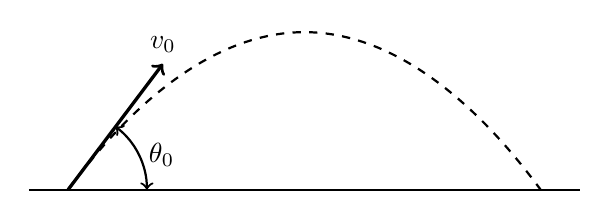
\begin{tikzpicture}
        %% NOTE: useful reference
        %% a = 2/9
        %% y = a x^2
        %% dy/dx = 2 a x
        %% theta = atan( dy/dx )
        \draw[thick] (-3.5,0) -- (3.5,0);
        \draw[thick,dashed] (-3,0) parabola bend (0,2) (3,0);
        \draw[very thick,->] (-3,0) -- ++ (53:2.0cm) node[pos=1.0,anchor=south] {$v_0$};
        \draw[thick,<->] (-2,0) arc (0:53:1cm) node[pos=0.5,anchor=west] {$\theta_0$};
    \end{tikzpicture}
    \end{center}
    Which of the following pairs of graphs best represents the vertical components of the velocity and acceleration,
        respectively, of the projectile as functions of time?
    \begin{choices}
        \AMCboxDimensions{down=-0.120\columnwidth}
        \wrongchoice{
            \begin{tikzpicture}
            \begin{groupplot}[
                    group style={group size=2 by 1},
                    axis line style={->},
                    axis y line=left,
                    axis x line=middle,
                    xtick=\empty,
                    ytick=\empty,
                    width=0.5\columnwidth,
                    height=0.309\columnwidth,
                    xmin=0,xmax=10,ymin=-10,ymax=10,
                ]
                \nextgroupplot[
                    xlabel={time},
                    ylabel={displacement},
                ] \addplot[thick,domain=0:10] {8 - 1.6*x};
                \nextgroupplot[
                    xlabel={time},
                    ylabel={acceleration},
                ] \addplot[thick,domain=0:10] {8 - 1.6*x};
            \end{groupplot}
            \end{tikzpicture}
        }
        \wrongchoice{
            \begin{tikzpicture}
            \begin{groupplot}[
                    group style={group size=2 by 1},
                    axis line style={->},
                    axis y line=left,
                    axis x line=middle,
                    xtick=\empty,
                    ytick=\empty,
                    width=0.5\columnwidth,
                    height=0.309\columnwidth,
                    xmin=0,xmax=10,ymin=-10,ymax=10,
                ]
                \nextgroupplot[
                    xlabel={time},
                    ylabel={displacement},
                ] \addplot[thick,domain=0:10] {8 - 1.6*x};
                \nextgroupplot[
                    x label style={anchor=north east},
                    xlabel={time},
                    ylabel={acceleration},
                ] \addplot[thick,domain=0:10] {-8 + 1.6*x};
            \end{groupplot}
            \end{tikzpicture}
        }
        \wrongchoice{
            \begin{tikzpicture}
            \begin{groupplot}[
                    group style={group size=2 by 1},
                    axis line style={->},
                    axis y line=left,
                    axis x line=middle,
                    xtick=\empty,
                    ytick=\empty,
                    width=0.5\columnwidth,
                    height=0.309\columnwidth,
                    xmin=0,xmax=10,ymin=-10,ymax=10,
                ]
                \nextgroupplot[
                    x label style={anchor=north east},
                    xlabel={time},
                    ylabel={displacement},
                ] \addplot[thick,domain=0:10] {-8 + 1.6*x};
                \nextgroupplot[
                    xlabel={time},
                    ylabel={acceleration},
                ] \addplot[very thick,dashed,domain=0:10] {0};
            \end{groupplot}
            \end{tikzpicture}
        }
        %% NOTE: Ans is D
        \correctchoice{
            \begin{tikzpicture}
            \begin{groupplot}[
                    group style={group size=2 by 1},
                    axis line style={->},
                    axis y line=left,
                    axis x line=middle,
                    xtick=\empty,
                    ytick=\empty,
                    width=0.5\columnwidth,
                    height=0.309\columnwidth,
                    xmin=0,xmax=10,ymin=-10,ymax=10,
                ]
                \nextgroupplot[
                    xlabel={time},
                    ylabel={displacement},
                ] \addplot[thick,domain=0:10] {8 - 1.6*x};
                \nextgroupplot[
                    xlabel={time},
                    ylabel={acceleration},
                ] \addplot[thick,domain=0:10] {-8};
            \end{groupplot}
            \end{tikzpicture}
        }
        \wrongchoice{
            \begin{tikzpicture}
            \begin{groupplot}[
                    group style={group size=2 by 1},
                    axis line style={->},
                    axis y line=left,
                    axis x line=middle,
                    xtick=\empty,
                    ytick=\empty,
                    width=0.5\columnwidth,
                    height=0.309\columnwidth,
                    xmin=0,xmax=10,ymin=-10,ymax=10,
                ]
                \nextgroupplot[
                    xlabel={time},
                    ylabel={displacement},
                ] \addplot[thick,domain=0:10] {8};
                \nextgroupplot[
                    xlabel={time},
                    ylabel={acceleration},
                ] \addplot[thick,domain=0:10] {0};
            \end{groupplot}
            \end{tikzpicture}
        }
    \end{choices}
\end{question}
}

\element{AP}{
\begin{question}{kinematics-Q12}
    An object is released from rest on a planet that has no atmosphere.
    The object falls freely for \SI{3.0}{\meter} in the first second.
    What is the magnitude of the acceleration due to gravity on the planet?
    \begin{multicols}{3}
    \begin{choices}
        \wrongchoice{\SI{1.5}{\meter\per\second\squared}}
        \wrongchoice{\SI{3.0}{\meter\per\second\squared}}
      \correctchoice{\SI{6.0}{\meter\per\second\squared}}
        \wrongchoice{\SI{10.0}{\meter\per\second\squared}}
        \wrongchoice{\SI{12.0}{\meter\per\second\squared}}
    \end{choices}
    \end{multicols}
\end{question}
}
       
\newcommand{\kinematicsQThirteen}{
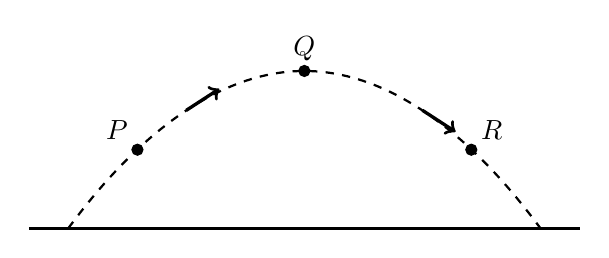
\begin{tikzpicture}
    \draw[thick] (-3.5,0) -- (3.5,0);
    %% NOTE: useful reference
    %% a = 2/9
    %% y = a x^2
    %% dy/dx = 2 a x
    %% theta = atan( dy/dx )
    \draw[thick,dashed] (-3,0) parabola bend (0,2) (3,0);
    %% Vectors
    \draw[very thick,->] (-1.5,1.5) -- ++ (+33:0.5);
    \draw[very thick,->] (+1.5,1.5) -- ++ (-33:0.5);
    %% Labels
    \draw[fill] (-2.12,1) circle (2pt) node[anchor=south east] {$P$};
    \draw[fill] (0,2) circle (2pt) node[anchor=south] {$Q$};
    \draw[fill] (+2.12,1) circle (2pt) node[anchor=south west] {$R$};
\end{tikzpicture}
}

\element{AP}{
\begin{question}{kinematics-Q13}
    A ball is thrown and follows the parabolic path shown above.
    Air friction is negligible.
    Point $Q$ is the highest point on the path.
    Points $P$ and $R$ are the same height above the ground.
    \begin{center}
        \kinematicsQThirteen
    \end{center}
    How do the speeds of the ball at the three points compare?
    \begin{multicols}{2}
    \begin{choices}
        \wrongchoice{$v_P < v_Q < v_R$}
        \wrongchoice{$v_R < v_Q < v_P$}
        \wrongchoice{$v_Q < v_R < v_P$}
      \correctchoice{$v_Q < v_P = v_R$}
        \wrongchoice{$v_P = v_R < v_Q$}
    \end{choices}
    \end{multicols}
\end{question}
}

\element{AP}{
\begin{question}{kinematics-Q14}
    A ball is thrown and follows the parabolic path shown above.
    Air friction is negligible.
    Point $Q$ is the highest point on the path.
    Points $P$ and $R$ are the same height above the ground.
    \begin{center}
        \kinematicsQThirteen
    \end{center}
    Which of the following diagrams best shows the direction of the acceleration of the ball at point $P$?
    \begin{multicols}{2}
    \begin{choices}
        \AMCboxDimensions{down=-0.8cm}
        \wrongchoice{
            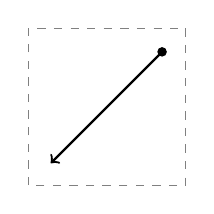
\begin{tikzpicture}
                \draw[dashed,draw=white!50!black] (+0.30,+0.30) rectangle (-1.7,-1.7);
                \draw[fill] (0,0) circle (1.5pt);
                \draw[thick,->] (0,0) -- (225:2.0cm);
            \end{tikzpicture}
        }
        \wrongchoice{
            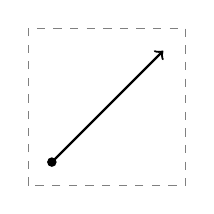
\begin{tikzpicture}
                \draw[dashed,draw=white!50!black] (-0.30,-0.30) rectangle (+1.7,+1.7);
                \draw[fill] (0,0) circle (1.5pt);
                \draw[thick,->] (0,0) -- (+45:2.0cm);
            \end{tikzpicture}
        }
        \wrongchoice{
            \begin{tikzpicture}
                \draw[dashed,draw=white!50!black] (0,-1) rectangle (+2.0,+1.0);
                \draw[fill] (0,0) circle (1.5pt);
                \draw[thick,->] (0,0) -- (0:2.0cm);
            \end{tikzpicture}
        }
        \wrongchoice{
            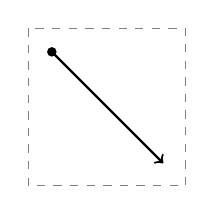
\begin{tikzpicture}
                \draw[dashed,draw=white!50!black] (-0.30,+0.30) rectangle (+1.7,-1.7);
                \draw[fill] (0,0) circle (1.5pt);
                \draw[thick,->] (0,0) -- (-45:2.0cm);
            \end{tikzpicture}
        }
        %% NOTE: ans is E
        \correctchoice{
            \begin{tikzpicture}
                \draw[dashed,draw=white!50!black] (-1,0) rectangle (1.0,-2.0);
                \draw[fill] (0,0) circle (1.5pt);
                \draw[thick,->] (0,0) -- (270:2.0cm);
            \end{tikzpicture}
        }
    \end{choices}
    \end{multicols}
\end{question}
}

\element{AP}{
\begin{question}{kinematics-Q15}
    A rock of mass $m$ is thrown horizontally off a building from a height $h$,
        as shown below.
    \begin{center}
    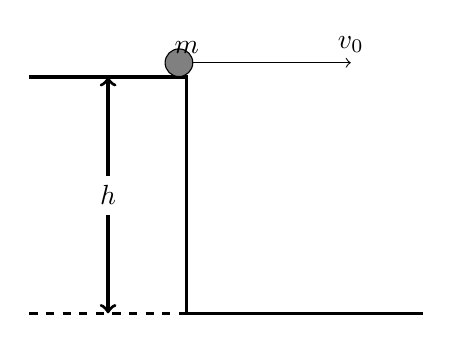
\begin{tikzpicture}[yscale=0.75]
        \draw[very thick] (-2,0) -- (0,0) -- (0,-4) -- (3,-4);
        %\draw (0.2,0.0) circle (3pt) node[anchor=south] {$m$};
        %\draw[thick,->] (0.2,0) -- ++ (0:1)
        %    node[pos=1.0,anchor=south] {$v_0$};
        \node[draw,fill=white!50!black,circle,anchor=south,minimum size=1em] (A) at (-0.1,0) {};
        \node[anchor=south,yshift=0.5em] (A.north) {$m$};
        \draw[->] (A.east) -- ++(0:2) node[pos=1.0,anchor=south] {$v_0$};
        \draw[very thick,dashed] (-2,-4) -- (0,-4);
        \node (A) at (-1,-2.0) {$h$};
        \draw[very thick,->] (A) -- (-1,0);
        \draw[very thick,->] (A) -- (-1,-4);
    \end{tikzpicture}
    \end{center}
    The speed of the rock as it leaves the thrower's hand at the edge of the building is $v_0$.
    How much time does it take the rock to travel from the edge of the building to the ground?
    \begin{multicols}{3}
    \begin{choices}
        \wrongchoice{$\sqrt{hv_0}$}
        \wrongchoice{$\dfrac{h}{v_0}$}
        \wrongchoice{$\dfrac{hv_0}{g}$}
        \wrongchoice{$\dfrac{2h}{g}$}
      \correctchoice{$\sqrt{\dfrac{2h}{g}}$}
    \end{choices}
    \end{multicols}
\end{question}
}

\element{AP}{
\begin{question}{kinematics-Q16}
    A ball is thrown straight up in the air.
    When the ball reaches its highest point,
        which of the following is true?
    \begin{choices}
        %% NOTE: questionmult?
        \wrongchoice{It is in equilibrium.}
        \wrongchoice{It has zero acceleration.}
        \wrongchoice{It has maximum momentum.}
        \wrongchoice{It has maximum kinetic energy.}
      \correctchoice{None of the provided.}
    \end{choices}
\end{question}
}

\element{AP}{
\begin{question}{kinematics-Q17}
    The graph below represents position versus time for an object being acted on by a constant force.
    \begin{center}
    \begin{tikzpicture}
        \begin{axis}[
            axis y line=left,
            axis x line=bottom,
            axis line style={->},
            xlabel={time},
            x unit=\si{\second},
            xtick={0,1,2,3},
            ylabel={position},
            y unit=\si{\meter},
            ytick={0,4,8,12,16,20},
            minor y tick num=1,
            grid=major,
            xmin=0,xmax=3.1,
            ymin=0,ymax=21,
            width=0.95\columnwidth,
            height=0.50\columnwidth,
        ]
        \addplot[line width=1pt,domain=0:3]{2*x*x};
        \end{axis}
    \end{tikzpicture}
    \end{center}
    The average speed during the interval between \SI{1}{\second} and \SI{2}{\second} is most nearly:
    \begin{multicols}{3}
    \begin{choices}
        \wrongchoice{\SI{2}{\meter\per\second}}
        \wrongchoice{\SI{4}{\meter\per\second}}
        \wrongchoice{\SI{5}{\meter\per\second}}
      \correctchoice{\SI{6}{\meter\per\second}}
        \wrongchoice{\SI{8}{\meter\per\second}}
    \end{choices}
    \end{multicols}
\end{question}
}

\element{AP}{
\begin{question}{kinematics-Q18}
    An object slides off a roof \SI{10}{\meter} above the ground with an initial horizontal speed of \SI{5}{\meter\per\second} as shown below.
    \begin{center}
        %% NOTE: this was copied from elsewhere
    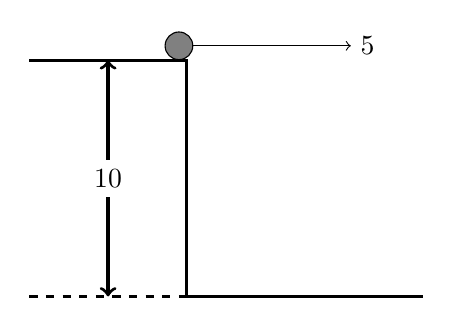
\begin{tikzpicture}[yscale=0.75]
        \draw[very thick] (-2,0) -- (0,0) -- (0,-4) -- (3,-4);
        %\draw (0.2,0.0) circle (3pt) node[anchor=south] {$m$};
        %\draw[thick,->] (0.2,0) -- ++ (0:1)
        %    node[pos=1.0,anchor=south] {$v_0$};
        \node[draw,fill=white!50!black,circle,anchor=south,minimum size=1em] (A) at (-0.1,0) {};
        \draw[->] (A.east) -- ++(0:2) node[pos=1.0,anchor=west] {\SI{5}{\meter\per\second}};
        \draw[very thick,dashed] (-2,-4) -- (0,-4);
        \node (A) at (-1,-2.0) {\SI{10}{\meter}};
        \draw[very thick,->] (A) -- (-1,0);
        \draw[very thick,->] (A) -- (-1,-4);
    \end{tikzpicture}
    \end{center}
    The time between the object's leaving the roof and hitting the ground is most nearly:
    \begin{multicols}{3}
    \begin{choices}
        \wrongchoice{\SI[parse-numbers=false]{\dfrac{1}{2}}{\second}}
        \wrongchoice{\SI[parse-numbers=false]{\dfrac{1}{\sqrt{2}}}{\second}}
      \correctchoice{\SI[parse-numbers=false]{\sqrt{2}}{\second}}
        \wrongchoice{\SI[parse-numbers=false]{2}{\second}}
        \wrongchoice{\SI[parse-numbers=false]{5\sqrt{2}}{\second}}
    \end{choices}
    \end{multicols}
\end{question}
}

\newcommand{\kinematicsQNineteen}{
\begin{tikzpicture}
    \begin{axis}[
        axis y line=left,
        axis x line=bottom,
        axis line style={->},
        xlabel={time},
        x unit=\si{\second},
        xtick={0,10,20,30,40},
        ylabel={velocity},
        y unit=\si{\meter\per\second},
        ytick={0,10},
        yticklabels={0,$v_0$},
        grid=major,
        xmin=0,xmax=42,
        ymin=0,ymax=20,
        width=0.95\columnwidth,
        height=0.45\columnwidth,
    ]
    %% NOTE: add text along curve?
    \addplot[line width=1pt,domain=0:40]{0.5*x}
        node[pos=0.1,anchor=south west] {Car $X$};
    \addplot[line width=1pt,domain=0:40]{10}
        node[pos=0.1,anchor=south west] {Car $X$};
    \end{axis}
\end{tikzpicture}
}

\element{AP}{
\begin{question}{kinematics-Q19}
    At time $t=\SI{0}{\second}$, car $X$ traveling with speed $v_0$ passes car $Y$ which is just starting to move.
    Both cars then travel on two parallel lanes of the same straight road.
    The graphs of speed $v$ versus time $t$ for both cars are shown below.
    \begin{center}
        \kinematicsQNineteen
    \end{center}
    Which of the following is true at time $t=\SI{20}{\second}$?
    \begin{choices}
      \correctchoice{Car $Y$ is behind car $X$.}
        \wrongchoice{Car $Y$ is passing car $X$.}
        \wrongchoice{Car $Y$ is in front of car $X$.}
        \wrongchoice{Both cars have the same acceleration.}
        \wrongchoice{Car $X$ is accelerating faster than car $Y$.}
    \end{choices}
\end{question}
}

\element{AP}{
\begin{question}{kinematics-Q20}
    At time $t=\SI{0}{\second}$, car $X$ traveling with speed $v_0$ passes car $Y$ which is just starting to move.
    Both cars then travel on two parallel lanes of the same straight road.
    The graphs of speed $v$ versus time $t$ for both cars are shown below.
    \begin{center}
        \kinematicsQNineteen
    \end{center}
    From time $t=\SI{0}{\second}$ to time $t=\SI{40}{\second}$,
        the areas under both curves are equal.
    Therefore, which of the following is true at time $t=\SI{40}{\second}$?
    \begin{choices}
        \wrongchoice{Car $Y$ is behind car $X$.}
      \correctchoice{Car $Y$ is passing car $X$.}
        \wrongchoice{Car $Y$ is in front of car $X$.}
        \wrongchoice{Both cars have the same acceleration.}
        \wrongchoice{Car $X$ is accelerating faster than car $Y$.}
    \end{choices}
\end{question}
}

\element{AP}{
\begin{question}{kinematics-Q21}
    Which of the following pairs of graphs shows the distance traveled versus time and the speed versus time for an object uniformly accelerated from rest?
    \begin{choices}
        %% NOTE: ans is E
        \AMCboxDimensions{down=-0.120\columnwidth}
        \wrongchoice{
            \begin{tikzpicture}
            \begin{groupplot}[
                    group style={group size=2 by 1},
                    axis line style={->},
                    axis y line=left,
                    axis x line=bottom,
                    xtick=\empty,
                    ytick=\empty,
                    width=0.5\columnwidth,
                    xmin=0,xmax=10,ymin=0,ymax=10,
                ]
                \nextgroupplot[
                    xlabel={time},
                    ylabel={distance},
                ] \addplot[thick,domain=0:10] {10 - 0.1*(x-10)*(x-10)};
                \nextgroupplot[
                    xlabel={time},
                    ylabel={speed},
                ] \addplot[thick,domain=0:10] {x};
            \end{groupplot}
            \end{tikzpicture}
        }
        \wrongchoice{
            \begin{tikzpicture}
            \begin{groupplot}[
                    group style={group size=2 by 1},
                    axis line style={->},
                    axis y line=left,
                    axis x line=bottom,
                    xtick=\empty,
                    ytick=\empty,
                    width=0.5\columnwidth,
                    xmin=0,xmax=10,ymin=0,ymax=10,
                ]
                \nextgroupplot[
                    xlabel={time},
                    ylabel={distance},
                ] \addplot[thick,domain=0:10] {10 - 0.1*(x-10)*(x-10)};
                \nextgroupplot[
                    x label style={anchor=north east},
                    xlabel={time},
                    ylabel={speed},
                ] \addplot[thick,domain=0:10] {0.1*x*x};
            \end{groupplot}
            \end{tikzpicture}
        }
        \wrongchoice{
            \begin{tikzpicture}
            \begin{groupplot}[
                    group style={group size=2 by 1},
                    axis line style={->},
                    axis y line=left,
                    axis x line=bottom,
                    xtick=\empty,
                    ytick=\empty,
                    width=0.5\columnwidth,
                    xmin=0,xmax=10,ymin=0,ymax=10,
                ]
                \nextgroupplot[
                    x label style={anchor=north east},
                    xlabel={time},
                    ylabel={distance},
                ] \addplot[thick,domain=0:10] {x};
                \nextgroupplot[
                    xlabel={time},
                    ylabel={speed},
                ] \addplot[thick,domain=0:10] {0.1*x*x};
            \end{groupplot}
            \end{tikzpicture}
        }
        \wrongchoice{
            \begin{tikzpicture}
            \begin{groupplot}[
                    group style={group size=2 by 1},
                    axis line style={->},
                    axis y line=left,
                    axis x line=bottom,
                    xtick=\empty,
                    ytick=\empty,
                    width=0.5\columnwidth,
                    xmin=0,xmax=10,ymin=0,ymax=10,
                ]
                \nextgroupplot[
                    xlabel={time},
                    ylabel={distance},
                ] \addplot[thick,domain=0:10] {0.1*x*x};
                \nextgroupplot[
                    xlabel={time},
                    ylabel={speed},
                ] \addplot[thick,domain=0:10] {0.1*x*x};
            \end{groupplot}
            \end{tikzpicture}
        }
        \wrongchoice{
            \begin{tikzpicture}
            \begin{groupplot}[
                    group style={group size=2 by 1},
                    axis line style={->},
                    axis y line=left,
                    axis x line=bottom,
                    xtick=\empty,
                    ytick=\empty,
                    width=0.5\columnwidth,
                    xmin=0,xmax=10,ymin=0,ymax=10,
                ]
                \nextgroupplot[
                    xlabel={time},
                    ylabel={distance},
                ] \addplot[thick,domain=0:10] {0.1*x*x};
                \nextgroupplot[
                    xlabel={time},
                    ylabel={speed},
                ] \addplot[thick,domain=0:10] {x};
            \end{groupplot}
            \end{tikzpicture}
        }
    \end{choices}
\end{question}
}

\element{AP}{
\begin{question}{kinematics-Q22}
    An object released from rest at time $t=\SI{0}{\second}$ slides down a frictionless incline a distance of \SI{1}{\meter} during the first second.
    The distance traveled by the object during the time interval from $t=\SI{1}{\second}$ to $t=\SI{2}{\second}$ is:
    \begin{multicols}{3}
    \begin{choices}
        \wrongchoice{\SI{1}{\meter}}
        \wrongchoice{\SI{2}{\meter}}
      \correctchoice{\SI{3}{\meter}}
        \wrongchoice{\SI{4}{\meter}}
        \wrongchoice{\SI{5}{\meter}}
    \end{choices}
    \end{multicols}
\end{question}
}

\element{AP}{
\begin{question}{kinematics-Q23}
    Two people are in a boat that is capable of a maximum speed of \SI{5}{\kilo\meter\per\hour} in still water,
        and wish to cross a river \SI{1}{\kilo\meter} wide to a point directly across from their starting point.
    If the speed of the water in the river is \SI{5}{\kilo\meter\per\hour},
        how much time is required for the crossing?
    \begin{multicols}{2}
    \begin{choices}
        \wrongchoice{\SI{0.05}{\hour}}
        \wrongchoice{\SI{0.1}{\hour}}
        \wrongchoice{\SI{1}{\hour}}
        \wrongchoice{\SI{10}{\hour}}
      \correctchoice{The point directly across from the starting point cannot be reached under these conditions.}
    \end{choices}
    \end{multicols}
\end{question}
}

\element{AP}{
\begin{question}{kinematics-Q24}
    A projectile is fired from the surface of the Earth with a speed of \SI{200}{\meter\per\second} at an angle of \ang{30} above the horizontal.
    If the ground is level,
        what is the maximum height reached by the projectile?
    \begin{multicols}{3}
    \begin{choices}
        \wrongchoice{\SI{5}{\meter}}
        \wrongchoice{\SI{10}{\meter}}
      \correctchoice{\SI{500}{\meter}}
        \wrongchoice{\SI{1 000}{\meter}}
        \wrongchoice{\SI{2 000}{\meter}}
    \end{choices}
    \end{multicols}
\end{question}
}

\element{AP}{
\begin{question}{kinematics-Q25}
    Vectors $\mathbf{V}_1$ and $\mathbf{V}_2$ shown below have equal magnitudes.
    \begin{center}
    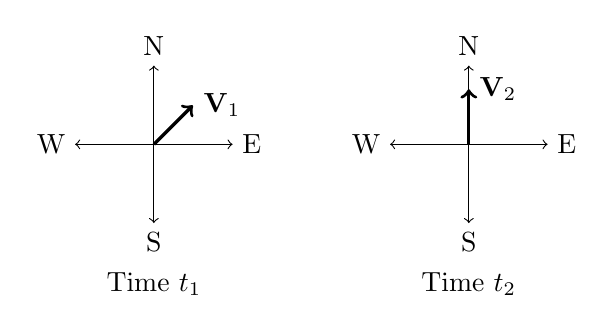
\begin{tikzpicture}
        \node (One) at (-2,0) {};
        \node (Two) at (+2,0) {};
        %% Left compass
        \draw[very thick,->] (One.center) -- ++ (45:0.7) node[pos=1.0,anchor=west] {$\mathbf{V}_1$};
        \draw (One) ++ (270:1.5) node[anchor=north] {Time $t_1$};
        \draw[->] (One.center) -- ++ (0:1) node[pos=1.0,anchor=west] {E};
        \draw[->] (One.center) -- ++ (90:1) node[pos=1.0,anchor=south] {N};
        \draw[->] (One.center) -- ++ (180:1) node[pos=1.0,anchor=east] {W};
        \draw[->] (One.center) -- ++ (270:1) node[pos=1.0,anchor=north] {S};
        %% Right compass
        \draw[very thick,->] (Two.center) -- ++ (90:0.7) node[pos=1.0,anchor=west] {$\mathbf{V}_2$};
        \draw (Two) ++ (270:1.5) node[anchor=north] {Time $t_2$};
        \draw[->] (Two.center) -- ++ (0:1) node[pos=1.0,anchor=west] {E};
        \draw[->] (Two.center) -- ++ (90:1) node[pos=1.0,anchor=south] {N};
        \draw[->] (Two.center) -- ++ (180:1) node[pos=1.0,anchor=east] {W};
        \draw[->] (Two.center) -- ++ (270:1) node[pos=1.0,anchor=north] {S};
    \end{tikzpicture}
    \end{center}
    The vectors represent the velocities of an object at times $t_1$, and $t_2$, respectively.
    The average acceleration of the object between time $t_1$ and $t_2$ was:
    \begin{multicols}{2}
    \begin{choices}
        \wrongchoice{zero }
        \wrongchoice{directed north}
        \wrongchoice{directed west}
        \wrongchoice{directed north of east}
      \correctchoice{directed north of west}
    \end{choices}
    \end{multicols}
\end{question}
}

\element{AP}{
\begin{question}{kinematics-Q26}
    A rock is dropped from the top of a \SI{45}{\meter} tower,
        and at the same time a ball is thrown from the top of the tower in a horizontal direction.
    Air resistance is negligible.
    The ball and the rock hit the level ground a distance of \SI{30}{\meter} apart.
    The horizontal velocity of the ball thrown was most nearly:
    \begin{multicols}{3}
    \begin{choices}
        \wrongchoice{\SI{5}{\meter\per\second}}
      \correctchoice{\SI{10}{\meter\per\second}}
        \wrongchoice{\SI{14.1}{\meter\per\second}}
        \wrongchoice{\SI{20}{\meter\per\second}}
        \wrongchoice{\SI{28.3}{\meter\per\second}}
    \end{choices}
    \end{multicols}
\end{question}
}

\element{AP}{
\begin{question}{kinematics-Q27}
    In the absence of air friction,
        an object dropped near the surface of the Earth experiences a constant acceleration of about \SI{9.8}{\meter\per\second\squared}.
    This means that the:
    \begin{choices}
      \correctchoice{speed of the object increases \SI{9.8}{\meter\per\second} during each second}
        \wrongchoice{speed of the object as it falls is \SI{9.8}{\meter\per\second}}
        \wrongchoice{object falls 9.8 meters during each second}
        \wrongchoice{object falls 9.8 meters during the first second only}
        \wrongchoice{rate of change of the displacement with respect to time for the object equals \SI{9.8}{\meter\per\second\squared}}
    \end{choices}
\end{question}
}

\element{AP}{
\begin{question}{kinematics-Q28}
    A \SI{500}{\kilo\gram} sports car accelerates uniformly from rest,
        reaching a speed of \SI{30}{\meter\per\second} in \SI{6}{\second}.
    During the \SI{6}{\second},
        the car has traveled a distance of:
    \begin{multicols}{3}
    \begin{choices}
        \wrongchoice{\SI{15}{\meter}}
        \wrongchoice{\SI{30}{\meter}}
        \wrongchoice{\SI{60}{\meter}}
      \correctchoice{\SI{90}{\meter}}
        \wrongchoice{\SI{180}{\meter}}
    \end{choices}
    \end{multicols}
\end{question}
}

\element{AP}{
\begin{question}{kinematics-Q29}
    %%*29.
    At a particular instant, a stationary observer on the ground sees a package falling with speed $v_1$ at an angle to the vertical.
    To a pilot flying horizontally at constant speed relative to the ground, the package appears to be falling vertically with a speed $v_2$ at that instant.
    What is the speed of the pilot relative to the ground?
    \begin{multicols}{2}
    \begin{choices}
        \wrongchoice{$v_1 + v-2$}
        \wrongchoice{$v_1 - v_2$}
        \wrongchoice{$v_2 - v_1$}
      \correctchoice{$\sqrt{v_1^2 - v_2^2}$}
        \wrongchoice{$\sqrt{v_1^2 + v_2^2}$}
    \end{choices}
    \end{multicols}
\end{question}
}

\element{AP}{
\begin{question}{kinematics-Q30}
    An object is shot vertically upward into the air with a positive initial velocity.
    Which of the following correctly describes the velocity and acceleration of the object at its maximum elevation?
    \begin{choices}
        %% NOTE: table format?
        %% Velocity Acceleration
        \wrongchoice{Positive Positive}
        \wrongchoice{Zero Zero}
        \wrongchoice{Negative Negative}
      \correctchoice{Zero Negative}
        \wrongchoice{Positive Negative}
    \end{choices}
\end{question}
}

\element{AP}{
\begin{question}{kinematics-Q31}
    A spring-loaded gun can fire a projectile to a height $h$ if it is fired straight up.
    If the same gun is pointed at an angle of \ang{45} from the vertical,
        what maximum height can now be reached by the projectile?
    \begin{multicols}{3}
    \begin{choices}
        \wrongchoice{$\dfrac{h}{4}$}
        \wrongchoice{$\dfrac{h}{2\sqrt{2}}$}
      \correctchoice{$\dfrac{h}{2}$}
        \wrongchoice{$\dfrac{h}{\sqrt{2}}$}
        \wrongchoice{$h$}
    \end{choices}
    \end{multicols}
\end{question}
}

\element{AP}{
\begin{question}{kinematics-Q32}
    A ball is thrown and follows a parabolic path, as shown below.
    \begin{center}
        \kinematicsQThirteen
    \end{center}
    Air friction is negligible.
    Point $Q$ is the highest point on the path.
    Which of the following best indicates the direction of the acceleration,
        if any, of the ball at point $Q$?
    \begin{multicols}{2}
    \begin{choices}
        \AMCboxDimensions{down=-1.0cm}
        \wrongchoice{
            \begin{tikzpicture}
                \draw[dashed,draw=white!50!black] (0,-1) rectangle (+2.0,+1.0);
                \draw[fill] (0,0) circle (1.5pt);
                \draw[thick,->] (0,0) -- (0:2.0cm);
            \end{tikzpicture}
        }
        \wrongchoice{
            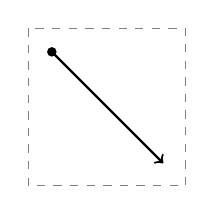
\begin{tikzpicture}
                \draw[dashed,draw=white!50!black] (-0.30,+0.30) rectangle (+1.7,-1.7);
                \draw[fill] (0,0) circle (1.5pt);
                \draw[thick,->] (0,0) -- (-45:2.0cm);
            \end{tikzpicture}
        }
        %% NOTE: ans is C
        \correctchoice{
            \begin{tikzpicture}
                \draw[dashed,draw=white!50!black] (-1.00,0.00) rectangle (+1.0,-2.0);
                \draw[fill] (0,0) circle (1.5pt);
                \draw[thick,->] (0,0) -- (270:2.0cm);
            \end{tikzpicture}
        }
        \wrongchoice{
            \begin{tikzpicture}
                \draw[dashed,draw=white!50!black] (-2.00,-1.00) rectangle (0.0,+1.0);
                \draw[fill] (0,0) circle (1.5pt);
                \draw[thick,->] (0,0) -- (180:2.0cm);
            \end{tikzpicture}
        }
        \wrongchoice{
            \begin{tikzpicture}
                \draw[dashed,draw=white!50!black] (-1.00,-1.00) rectangle (+1.0,+1.0);
                \draw[fill] (0,0) circle (1.5pt)
                    node[anchor=south] {$\vec{a}=0$};
            \end{tikzpicture}
        }
        %\wrongchoice{There is no acceleration of the ball at point $Q$.}
    \end{choices}
    \end{multicols}
\end{question}
}

\element{AP}{
\begin{question}{kinematics-Q33}
    The velocity of a projectile at launch has a horizontal component $v_h$ and a vertical component $v_v$.
    Air resistance is negligible.
    When the projectile is at the highest point of its trajectory,
        which of the following shows the vertical and horizontal components of its velocity and the vertical component of its acceleration?
    %% NOTE: Tabular answers
    \begin{multicols}{2}
    \begin{choices}
        %% NOTE: ans is E
        \wrongchoice{ }
    \end{choices}
    \end{multicols}
\end{question}
}

\element{AP}{
\begin{question}{kinematics-Q34}
    The graph below shows the velocity $v$ as a function of time $t$ for an object moving in a straight line.
    \begin{center}
    \begin{tikzpicture}
        \begin{axis}[
            axis y line=left,
            axis x line=bottom,
            axis line style={->},
            xlabel={time},
            xtick=\empty,
            ylabel={velocity},
            ytick=\empty,
            xmin=0,xmax=3,
            ymin=0,ymax=1,
            width=0.95\columnwidth,
            height=0.40\columnwidth,
        ]
        \addplot[line width=1pt,domain=0:1]{x};
        \addplot[line width=1pt,domain=1:3]{1};
        \addplot[line width=1pt,domain=3:4]{3-x};
        \end{axis}
    \end{tikzpicture}
    \end{center}
    Which of the following graphs shows the corresponding displacement as a function of time for the same time interval?
    \begin{multicols}{2}
    \begin{choices}
        %% NOTE: ans is D
        %% NOTE: finish this
        \AMCboxDimensions{down=-2.5em}
        \wrongchoice{
            \begin{tikzpicture}[font=\small]
                \begin{axis}[
                    axis y line=left,
                    axis x line=middle,
                    axis line style={->},
                    xlabel={time},
                    xtick=\empty,
                    ylabel={displacement},
                    xtick=\empty,
                    xmin=0,xmax=3,
                    ymin=0,ymax=1,
                    width=0.95\columnwidth,
                    very thin,
                ]
                \addplot[line width=1pt,domain=0:1]{1-(x-1)*(x-1)};
                \addplot[line width=1pt,domain=1:3]{1};
                \addplot[line width=1pt,domain=3:4]{1-(x-3)*(x-3)};
                \end{axis}
            \end{tikzpicture}
        }
        \wrongchoice{
            \begin{tikzpicture}[font=\small]
                \begin{axis}[
                    axis y line=left,
                    axis x line=middle,
                    axis line style={->},
                    xlabel={time},
                    xtick=\empty,
                    ylabel={displacement},
                    xtick=\empty,
                    xmin=0,xmax=3,
                    ymin=0,ymax=1,
                    width=0.95\columnwidth,
                    very thin,
                ]
                \addplot[line width=1pt,domain=0:1]{x*x};
                \addplot[line width=1pt,domain=1:3]{1};
                \addplot[line width=1pt,domain=3:4]{(x-4)*(x-4)};
                \end{axis}
            \end{tikzpicture}
        }
        \wrongchoice{
            \begin{tikzpicture}[font=\small]
                \begin{axis}[
                    axis y line=left,
                    axis x line=middle,
                    axis line style={->},
                    xlabel={time},
                    xtick=\empty,
                    ylabel={displacement},
                    xtick=\empty,
                    xmin=0,xmax=3,
                    ymin=0,ymax=1,
                    width=0.95\columnwidth,
                    very thin,
                ]
                \addplot[domain=0:4]{0.25 * x^2};
                \addplot[domain=4:8,dashed]{4 + 2*(x-4)};
                \addplot[domain=8:12]{-20 + 6*x - 0.25*x^2};
                \end{axis}
            \end{tikzpicture}
        }
        \wrongchoice{
            \begin{tikzpicture}
                \begin{axis}[
                    xlabel={$t$},
                    ylabel={$v$},
                    xtick=\empty,
                    ytick=\empty,
                    xmin=0,xmax=12,
                    ymin=0,ymax=5,
                    width=\columnwidth,
                    height=0.618\columnwidth,
                ]
                \addplot[domain=0:4]{0.5 * x};
                \addplot[domain=4:8]{2};
                \addplot[domain=8:12]{2 - 0.5*(x-8)};
                \end{axis}
            \end{tikzpicture}
        }
        \wrongchoice{
            \begin{tikzpicture}
                \begin{axis}[
                    xlabel={$t$},
                    ylabel={$v$},
                    xtick=\empty,
                    ytick=\empty,
                    xmin=0,xmax=12,
                    ymin=0,ymax=5,
                    width=\columnwidth,
                    height=0.618\columnwidth,
                ]
                \addplot[domain=0:4]{5 - 0.5 *x};
                \addplot[domain=4:8]{3};
                \addplot[domain=8:12]{3 - 0.5*(x-8)};
                \end{axis}
            \end{tikzpicture}
        }
        \wrongchoice{
            \begin{tikzpicture}
                \begin{axis}[
                    xlabel={$t$},
                    ylabel={$v$},
                    xtick=\empty,
                    ytick=\empty,
                    xmin=0,xmax=12,
                    ymin=0,ymax=5,
                    width=\columnwidth,
                    height=0.618\columnwidth,
                ]
                \addplot[domain=0:4]{1};
                \addplot[domain=4:8]{1 + 0.75*(x-4)};
                \addplot[domain=8:12]{4};
                \end{axis}
            \end{tikzpicture}
        }
        \wrongchoice{
            \begin{tikzpicture}
                \begin{axis}[
                    xlabel={$t$},
                    ylabel={$v$},
                    xtick=\empty,
                    ytick=\empty,
                    xmin=0,xmax=12,
                    ymin=0,ymax=5,
                    width=\columnwidth,
                    height=0.618\columnwidth,
                ]
                \addplot[domain=0:4]{4};
                \addplot[domain=4:8]{4 - 0.75*(x-4)};
                \addplot[domain=8:12]{1};
                \end{axis}
            \end{tikzpicture}
        }
        \wrongchoice{
            \begin{tikzpicture}
                \begin{axis}[
                    xlabel={$t$},
                    ylabel={$v$},
                    xtick=\empty,
                    ytick=\empty,
                    xmin=0,xmax=12,
                    ymin=0,ymax=5,
                    width=\columnwidth,
                    height=0.618\columnwidth,
                ]
                \addplot[domain=0:4]{0.5 * x};
                \addplot[domain=4:8]{2};
                \addplot[domain=8:12]{2 + 0.5*(x-8)};
                \end{axis}
            \end{tikzpicture}
        }
        \wrongchoice{
            \begin{tikzpicture}
                \begin{axis}[
                    xlabel={$t$},
                    ylabel={$v$},
                    xtick=\empty,
                    ytick=\empty,
                    xmin=0,xmax=12,
                    ymin=0,ymax=5,
                    width=\columnwidth,
                    height=0.618\columnwidth,
                ]
                \addplot[domain=0:4]{0.125 * x};
                \addplot[domain=4:8]{0.5 + 0.75*(x-4)};
                \addplot[domain=8:12]{3.5 + 0.125*(x-8)};
                \end{axis}
            \end{tikzpicture}
        }
    \end{choices}
    \end{multicols}
\end{question}
}

\element{AP}{
\begin{question}{kinematics-Q35}
    An object is dropped from rest from the top of a \SI{400}{\meter} cliff on Earth.
    If air resistance is negligible,
        what is the distance the object travels during the first \SI{6}{\second} of its fall?
    \begin{multicols}{3}
    \begin{choices}
        \wrongchoice{\SI{30}{\meter}}
        \wrongchoice{\SI{60}{\meter}}
        \wrongchoice{\SI{120}{\meter}}
      \correctchoice{\SI{180}{\meter}}
        \wrongchoice{\SI{360}{\meter}}
    \end{choices}
    \end{multicols}
\end{question}
}

\element{AP}{
\begin{question}{kinematics-Q36}
    A target $T$ lies flat on the ground \SI{3}{\meter} from the side of a building that is \SI{10}{\meter} tall,
        as shown below.
    \begin{center}
        %% NOTE: this was copied from elsewhere
    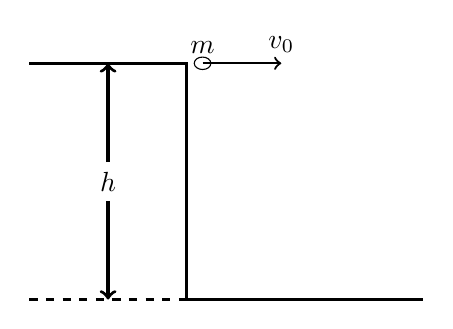
\begin{tikzpicture}[yscale=0.75]
        \draw[very thick] (-2,0) -- (0,0) -- (0,-4) -- (3,-4);
        \draw (0.2,0.0) circle (3pt) node[anchor=south] {$m$};
        \draw[thick,->] (0.2,0) -- ++ (0:1)
            node[pos=1.0,anchor=south] {$v_0$};
        \draw[very thick,dashed] (-2,-4) -- (0,-4);
        \node (A) at (-1,-2.0) {$h$};
        \draw[very thick,->] (A) -- (-1,0);
        \draw[very thick,->] (A) -- (-1,-4);
    \end{tikzpicture}
    \end{center}
    A student rolls a ball off the horizontal roof of the building in the direction of the target.
    Air resistance is negligible.
    The horizontal speed with which the ball must leave the roof if it is to strike the target is most nearly:
    \begin{multicols}{3}
    \begin{choices}
        \wrongchoice{\SI[parse-numbers=false]{\frac{3}{10}}{\meter\per\second}}
        \wrongchoice{\SI[parse-numbers=false]{\sqrt{2}}{\meter\per\second}}
      \correctchoice{\SI[parse-numbers=false]{\frac{3}{\sqrt{2}}}{\meter\per\second}}
        \wrongchoice{\SI[parse-numbers=false]{\frac{3}{\sqrt{2}}}{\meter\per\second}}
        \wrongchoice{\SI[parse-numbers=false]{10\sqrt{\frac{5}{3}}}{\meter\per\second}}
    \end{choices}
    \end{multicols}
\end{question}
}

\element{AP}{
\begin{question}{kinematics-Q37}
    The graph below shows velocity $v$ versus time $t$ for an object in linear motion.
    \begin{center}
        %% NOTE; copied from eleswhere, need to finish
    \begin{tikzpicture}
        \begin{axis}[
            axis y line=left,
            axis x line=bottom,
            axis line style={->},
            xlabel={time},
            x unit=\si{\second},
            xtick={0,1,2,3,4},
            ylabel={velocity},
            y unit=\si{\meter\per\second},
            ytick={-2,-1,0,1,2},
            grid=major,
            xmin=0,xmax=4.5,
            ymin=-2.5,ymax=2.5,
            width=0.95\columnwidth,
            height=0.50\columnwidth,
        ]
        \addplot[line width=1pt,domain=0:0.5]{-2*x};
        \addplot[line width=1pt,domain=0.5:2]{-2 + 2*x};
        \addplot[line width=1pt,domain=2:3]{2};
        \addplot[line width=1pt,domain=3:4]{8 - 2*x};
        \end{axis}
    \end{tikzpicture}
    \end{center}
    Which of the following is a possible graph of position $x$ versus time $t$ for this object?
    \begin{multicols}{2}
    \begin{choices}
        %% NOTE: ans is A
        \wrongchoice{
            \begin{tikzpicture}
            \end{tikzpicture}
        }
    \end{choices}
    \end{multicols}
\end{question}
}

\element{AP}{
\begin{question}{kinematics-Q38}
    A student is testing the kinematic equations for uniformly accelerated
        motion by measuring the time it takes for light-weight plastic balls
        to fall to the floor from a height of \SI{3}{\meter} in the lab.
    The student predicts the time to fall using g as \SI{9.80}{\meter\per\second\squared}
        but finds the measured time to be \SI{35}{\percent} greater.
    Which of the following is the most likely cause of the large percent error?
    \begin{choices}
        \wrongchoice{The acceleration due to gravity is \SI{70}{\percent} greater than \SI{9.80}{\meter\per\second\squared} at this location.}
        \wrongchoice{The acceleration due to gravity is \SI{70}{\percent} less than \SI{9.80}{\meter\per\second\squared} at this location.}
        \wrongchoice{Air resistance increases the downward acceleration.}
      \correctchoice{The acceleration of the plastic balls is not uniform.}
        \wrongchoice{The plastic balls are not truly spherical.}
    \end{choices}
\end{question}
}

\element{AP}{
\begin{question}{kinematics-Q39}
    An object is thrown with velocity $v$ from the edge of a cliff above level ground.
    Neglect air resistance.
    \begin{center}
    \begin{tikzpicture}
        \draw[thick] (-2,0) -- (0,0) -- (0,-2) -- (3,-2);
        \draw[dashed,thick] (0,0) -- ++(0:2);
        \draw[<->] (1,0) arc (0:45:1) node[pos=0.5,anchor=west] {$\theta$};
        \draw[thick,->] (0,0) -- ++(45:2)
            node[pos=1.0,anchor=south west] {$\mathbf{v}$};
    \end{tikzpicture}
    \end{center}
    In order for the object to travel a maximum horizontal distance from the cliff before hitting the ground,
        the throw should be at an angle $\theta$ with respect to the horizontal of:
    \begin{choices}
        \wrongchoice{greater than \ang{60} above the horizontal}
        \wrongchoice{greater than \ang{45} but less than \ang{60} above the horizontal}
      \correctchoice{greater than zero but less than \ang{45} above the horizontal}
        \wrongchoice{zero}
        \wrongchoice{greater than zero but less than \ang{45} below the horizontal}
    \end{choices}
\end{question}
}

\element{AP}{
\begin{question}{kinematics-Q40}
    Starting from rest at time $t=\SI{0}{\second}$,
        a car moves in a straight line with an acceleration given by the accompanying graph.
    \begin{center}
    \begin{tikzpicture}
        \begin{axis}[
            axis y line=left,
            axis x line=bottom,
            axis line style={->},
            clip=false,
            xlabel={time},
            x unit=\si{\second},
            xtick={0,2,4,6},
            minor x tick num=1,
            ylabel={acceleration},
            y unit=\si{\meter\per\second\squared},
            minor y tick num=1,
            ytick={0,2,4,6},
            grid=major,
            xmin=0,xmax=6.5,
            ymin=0,ymax=6,
            width=0.90\columnwidth,
            height=0.45\columnwidth,
        ]
        \addplot[very thick,domain=0:5]{5-x};
        \addplot[very thick,domain=5:6]{0};
        \end{axis}
    \end{tikzpicture}
    \end{center}
    What is the speed of the car at $t=\SI{3}{\second}$?
    \begin{multicols}{3}
    \begin{choices}
        \wrongchoice{\SI{1.0}{\meter\per\second}}
        \wrongchoice{\SI{2.0}{\meter\per\second}}
        \wrongchoice{\SI{6.0}{\meter\per\second}}
      \correctchoice{\SI{10.5}{\meter\per\second}}
        \wrongchoice{\SI{12.5}{\meter\per\second}}
    \end{choices}
    \end{multicols}
\end{question}
}

\element{AP}{
\begin{question}{kinematics-Q41}
    A flare is dropped from a plane flying over level ground at a velocity of \SI{70}{\meter\per\second} in the horizontal direction.
    At the instant the flare is released,
        the plane begins to accelerate horizontally at \SI{0.75}{\meter\per\second\squared}.
    The flare takes \SI{4.0}{\second} to reach the ground.
    Assume air resistance is negligible.
    Relative to a spot directly under the flare at release,
        the flare lands:
    \begin{choices}
        \wrongchoice{directly on the spot.}
        \wrongchoice{\SI{6.0}{\meter} in front of the spot. }
        \wrongchoice{\SI{274}{\meter} in front of the spot.}
      \correctchoice{\SI{280}{\meter} in front of the spot.}
        \wrongchoice{\SI{286}{\meter} in front of the spot.}
    \end{choices}
\end{question}
}

\element{AP}{
\begin{question}{kinematics-Q42}
    A flare is dropped from a plane flying over level ground at a velocity of \SI{70}{\meter\per\second} in the horizontal direction.
    At the instant the flare is released,
        the plane begins to accelerate horizontally at \SI{0.75}{\meter\per\second\squared}.
    The flare takes \SI{4.0}{\second} to reach the ground.
    Assume air resistance is negligible.
    %As seen by the pilot of the plane (in question \#41) and measured relative to a spot directly under the plane when the flare lands, the flare lands
    As seen by the pilot of the plane and measured relative to a spot directly under the plane when the flare lands,
        the flare lands:
    \begin{choices}
        \wrongchoice{\SI{286}{\meter} behind the plane.}
      \correctchoice{\SI{6.0}{\meter} behind the plane.}
        \wrongchoice{directly under the plane.}
        \wrongchoice{\SI{12}{\meter} in front of the plane.}
        \wrongchoice{\SI{274}{\meter} in front of the plane}
    \end{choices}
\end{question}
}

\element{AP}{
\begin{question}{kinematics-Q43}
    The graph below is a plot of position versus time.
    \begin{center}
    \begin{tikzpicture}
    \end{tikzpicture}
    \end{center}
    For which labeled region is the velocity positive and the acceleration negative?
    \begin{multicols}{5}
    \begin{choices}[o]
        \wrongchoice{$A$}
        \wrongchoice{$B$}
        \wrongchoice{$C$}
        \wrongchoice{$D$}
      \correctchoice{$E$}
    \end{choices}
    \end{multicols}
\end{question}
}

\element{AP}{
\begin{question}{kinematics-Q44}
    A child left her home and started walking at a constant velocity.
    After a time she stopped for a while and then continued on with a velocity greater than she originally had.
    All of a sudden she turned around and walked very quickly back home.
    Which of the following graphs best represents the distance versus time graph for her walk?
    \begin{multicols}{5}
    \begin{choices}
        %% NOTE: ans is B
        %% NOTE: bezier curve?
        \wrongchoice{
            \begin{tikzpicture}
            \end{tikzpicture}
        }
    \end{choices}
    \end{multicols}
\end{question}
}

\element{AP}{
\begin{question}{kinematics-Q45}
    In a rescue attempt,
        a hovering helicopter drops a life preserver to a swimmer being swept downstream by a river current of constant velocity $v$.
    The helicopter is at a height of \SI{9.8}{\meter}.
    The swimmer is \SI{6.0}{\meter} upstream from a point directly under the helicopter when the life preserver is released.
    It lands \SI{2.0}{\meter} in front of the swimmer.
    How fast is the current flowing?
    Neglect air resistance.
    \begin{multicols}{3}
    \begin{choices}
        \wrongchoice{\SI{13.7}{\meter\per\second}}
        \wrongchoice{\SI{9.8}{\meter\per\second}}
        \wrongchoice{\SI{6.3}{\meter\per\second}}
      \correctchoice{\SI{2.8}{\meter\per\second}}
        \wrongchoice{\SI{2.4}{\meter\per\second}}
    \end{choices}
    \end{multicols}
\end{question}
}

\element{AP}{
\begin{question}{kinematics-Q46}
    A child tosses a ball directly upward.
    Its total time in the air is $T$.
    Its maximum height is $H$.
    What is its height after it has been in the air a time $T/4$?
    Neglect air resistance.
    \begin{multicols}{3}
    \begin{choices}
        \wrongchoice{$\dfrac{H}{4}$}
        \wrongchoice{$\dfrac{H}{3}$}
        \wrongchoice{$\dfrac{H}{2}$}
        \wrongchoice{$\dfrac{2H}{3}$}
      \correctchoice{$\dfrac{3H}{4}$}
    \end{choices}
    \end{multicols}
\end{question}
}

\element{AP}{
\begin{questionmult}{kinematics-Q47}
    A whiffle ball is tossed straight up, reaches a highest point, and falls back down.
    Air resistance is not negligible.
    Which of the following statements are true?
    \begin{choices}
      \correctchoice{The ball's speed is zero at the highest point.}
        \wrongchoice{The ball's acceleration is zero at the highest point.}
        \wrongchoice{The ball takes a longer time to travel up to the highest point than to fall back down.}
    \end{choices}
\end{questionmult}
}

\element{AP}{
\begin{question}{kinematics-Q48}
    A truck driver travels three-fourths the distance of his run at one velocity ($v$)
        and then completes his run at one half his original velocity ($1⁄2v$).
    What was the trucker's average speed for the trip?
    \begin{multicols}{3}
    \begin{choices}
        \wrongchoice{$0.85\,v$}
      \correctchoice{$0.80\,v$}
        \wrongchoice{$0.75\,v$}
        \wrongchoice{$0.70\,v$}
        \wrongchoice{$0.65\,v$}
    \end{choices}
    \end{multicols}
\end{question}
}

\element{AP}{
\begin{question}{kinematics-Q49}
    Below is a graph of the distance vs. time for car moving along a road.
    \begin{center}
    \begin{tikzpicture}
    \end{tikzpicture}
    \end{center}
    According the graph,
        at which of the following times would the automobile have been accelerating positively?
    \begin{choices}
        \wrongchoice{\SI{0}{\minute}, \SI{20}{\minute}, \SI{38}{\minute}, and \SI{60}{\minute}}
        \wrongchoice{\SI{5}{\minute}, \SI{12}{\minute}, \SI{29}{\minute}, and \SI{35}{\minute}}
      \correctchoice{\SI{5}{\minute}, \SI{29}{\minute}, and \SI{57}{\minute}}
        \wrongchoice{\SI{12}{\minute}, \SI{35}{\minute}, and \SI{41}{\minute}}
        \wrongchoice{at all times from \SI{0}{\minute} to \SI{60}{\minute}}
    \end{choices}
\end{question}
}

\element{AP}{
\begin{question}{kinematics-Q50}
    A large beach ball is dropped from the ceiling of a school gymnasium to the floor about \SI{10}{\meter} below.
    Which of the following graphs would best represent its velocity as a function of time?
    (do not neglect air resistance)
    \begin{multicols}{2}
    \begin{choices}
        \AMCboxDimensions{down=-2.5em}
        \wrongchoice{
            \begin{tikzpicture}
                \begin{axis}[
                    axis y line=left,
                    axis x line=bottom,
                    axis line style={->},
                    xlabel={time},
                    xtick=\empty,
                    ylabel={velocity},
                    ytick=\empty,
                    xmin=0,xmax=11,
                    ymin=0,ymax=11,
                    width=0.95\columnwidth,
                    very thin,
                ]
                \addplot[line width=1pt,domain=0:10]{x};
                \end{axis}
            \end{tikzpicture}
        }
        \wrongchoice{
            \begin{tikzpicture}
                \begin{axis}[
                    axis y line=left,
                    axis x line=bottom,
                    axis line style={->},
                    xlabel={time},
                    xtick=\empty,
                    ylabel={velocity},
                    ytick=\empty,
                    xmin=0,xmax=11,
                    ymin=0,ymax=11,
                    width=0.95\columnwidth,
                    very thin,
                ]
                \addplot[line width=1pt,domain=0:10]{0.1*x*x};
                \end{axis}
            \end{tikzpicture}
        }
        \wrongchoice{
            \begin{tikzpicture}
                \begin{axis}[
                    axis y line=left,
                    axis x line=bottom,
                    axis line style={->},
                    xlabel={time},
                    xtick=\empty,
                    ylabel={velocity},
                    ytick=\empty,
                    xmin=0,xmax=11,
                    ymin=0,ymax=11,
                    width=0.95\columnwidth,
                    very thin,
                ]
                \addplot[line width=1pt,domain=0:10]{0.05*x*x};
                \end{axis}
            \end{tikzpicture}
        }
        %% NOTE: ans is D
        \correctchoice{
            \begin{tikzpicture}
                \begin{axis}[
                    axis y line=left,
                    axis x line=bottom,
                    axis line style={->},
                    xlabel={time},
                    xtick=\empty,
                    ylabel={velocity},
                    ytick=\empty,
                    xmin=0,xmax=11,
                    ymin=0,ymax=11,
                    width=0.95\columnwidth,
                    very thin,
                ]
                \addplot[line width=1pt,domain=0:10]{10-0.1*(x-10)*(x-10)};
                \end{axis}
            \end{tikzpicture}
        }
        \wrongchoice{
            \begin{tikzpicture}
                \begin{axis}[
                    axis y line=left,
                    axis x line=bottom,
                    axis line style={->},
                    xlabel={time},
                    xtick=\empty,
                    ylabel={velocity},
                    ytick=\empty,
                    xmin=0,xmax=11,
                    ymin=0,ymax=11,
                    width=0.95\columnwidth,
                    very thin,
                ]
                \addplot[line width=1pt,domain=0:6]{1.5*x};
                \addplot[line width=1pt,domain=6:10]{9};
                \end{axis}
            \end{tikzpicture}
        }
    \end{choices}
    \end{multicols}
\end{question}
}

\newcommand{\kinematicsQFiftyOne}{
\begin{tikzpicture}
    \begin{axis}[
        axis y line=left,
        axis x line=middle,
        axis line style={->},
        xlabel={time},
        x unit=\si{\second},
        xtick={0,2,4,6,8},
        minor x tick num=1,
        ylabel={acceleration},
        y unit=\si{\meter\per\second\squared},
        ytick={-4,-2,0,2,4},
        xmin=0,xmax=8.5,
        ymin=-4.1,ymax=4.1,
        width=0.95\columnwidth,
        height=0.50\columnwidth,
    ]
    \addplot[line width=1pt,domain=0:2]{2*x};
    \addplot[line width=1pt,domain=2:6]{8 - 2*x};
    \addplot[line width=1pt,domain=6:8]{-16 + 2*x};
    \end{axis}
\end{tikzpicture}
}

\element{AP}{
\begin{question}{kinematics-Q51}
    % Questions 51 – 52
    A car starts from rest and accelerates as shown in the graph below.
    \begin{center}
        \kinematicsQFiftyOne
    \end{center}
    At what time would the car be moving with the greatest velocity?
    \begin{multicols}{3}
    \begin{choices}
        \wrongchoice{\SI{0}{\second}}
        \wrongchoice{\SI{2}{\second}}
      \correctchoice{\SI{4}{\second}}
        \wrongchoice{\SI{6}{\second}}
        \wrongchoice{\SI{8}{\second}}
    \end{choices}
    \end{multicols}
\end{question}
}

\element{AP}{
\begin{question}{kinematics-Q52}
    A car starts from rest and accelerates as shown in the graph below.
    \begin{center}
        \kinematicsQFiftyOne
    \end{center}
    At what time would the car be farthest from its original starting position?
    \begin{multicols}{3}
    \begin{choices}
        \wrongchoice{\SI{0}{\second}}
        \wrongchoice{\SI{2}{\second}}
        \wrongchoice{\SI{4}{\second}}
        \wrongchoice{\SI{6}{\second}}
      \correctchoice{\SI{8}{\second}}
    \end{choices}
    \end{multicols}
\end{question}
}

\element{AP}{
\begin{question}{kinematics-Q53}
    A ball is dropped \SI{1.0}{\meter} to the floor.
    If the speed of the ball as it rebounds from the floor is \SI{75}{\percent} of the speed at which it struck the floor,
        how high will the ball rise?
    \begin{multicols}{3}
    \begin{choices}
        \wrongchoice{\SI{0.28}{\meter}}
        \wrongchoice{\SI{0.35}{\meter}}
      \correctchoice{\SI{0.56}{\meter}}
        \wrongchoice{\SI{0.75}{\meter}}
        \wrongchoice{\SI{0.84}{\meter}}
    \end{choices}
    \end{multicols}
\end{question}
}

\element{AP}{
\begin{question}{kinematics-Q54}
    Which of the following sets of graphs might be the corresponding graphs of
        position $x$, velocity $v$, and acceleration $a$ vs. time $t$ for a moving particle?
    \begin{choices}
        \AMCboxDimensions{down=-2.5em}
        \wrongchoice{
            \begin{tikzpicture}[font=\small]
            \begin{groupplot}[
                    %% NOTE: anchor axis differently to optimize space
                    group style={group size=3 by 1},
                    width=0.33\columnwidth,
                    x label style={
                        at={(current axis.right of origin)},
                        anchor=west,
                    },
                    axis x line=middle,
                    xlabel={$t$},
                    xtick=\empty,
                    y label style={
                        at={(current axis.above origin)},
                        anchor=south,
                        rotate=270,
                    },
                    axis y line=left,
                    ytick=\empty,
                    ylabel=\empty,
                    xmin=0,xmax=11,
                    ymin=-10,ymax=10,
                ]
                \nextgroupplot[
                    ylabel={$x$},
                    ] \addplot[thick,domain=0:10] {x};
                \nextgroupplot[
                    ylabel={$v$},
                    ] \addplot[thick,domain=0:10] {5};
                \nextgroupplot[ 
                    ylabel={$a$},
                    ] \addplot[thick,domain=0:10] {10-x};
            \end{groupplot}
            \end{tikzpicture}
        }
        \wrongchoice{
            \begin{tikzpicture}[font=\small]
            \begin{groupplot}[
                    group style={group size=3 by 1},
                    width=0.33\columnwidth,
                    x label style={
                        at={(current axis.right of origin)},
                        anchor=west,
                    },
                    axis x line=middle,
                    xlabel={$t$},
                    xtick=\empty,
                    y label style={
                        at={(current axis.above origin)},
                        anchor=south,
                        rotate=270,
                    },
                    axis y line=left,
                    ytick=\empty,
                    ylabel=\empty,
                    xmin=0,xmax=11,
                    ymin=-10,ymax=10,
                ]
                \nextgroupplot[
                    ylabel={position},
                    ] \addplot[thick,domain=0:10] {10-x};
                \nextgroupplot[
                    ylabel={acceleration},
                    ] \addplot[thick,domain=0:10] {5};
                \nextgroupplot[ 
                    ylabel={acceleration},
                    ] \addplot[thick,domain=0:10] {-x};
            \end{groupplot}
            \end{tikzpicture}
        }
        %% NOTE: ans is C
        \correctchoice{
            \begin{tikzpicture}[font=\small]
            \begin{groupplot}[
                    group style={group size=3 by 1},
                    width=0.33\columnwidth,
                    x label style={
                        at={(current axis.right of origin)},
                        anchor=west,
                    },
                    axis x line=middle,
                    xlabel={$t$},
                    xtick=\empty,
                    y label style={
                        at={(current axis.above origin)},
                        anchor=south,
                        rotate=270,
                    },
                    axis y line=left,
                    ytick=\empty,
                    ylabel=\empty,
                    xmin=0,xmax=11,
                    ymin=-10,ymax=10,
                ]
                \nextgroupplot[
                    ylabel={position},
                    ] \addplot[thick,domain=0:10] {0.1*(x-10)*(x-10)};
                \nextgroupplot[
                    ylabel={acceleration},
                    ] \addplot[thick,domain=0:10] {10-0.8*x};
                \nextgroupplot[ 
                    ylabel={acceleration},
                    ] \addplot[thick,domain=0:10] {-5};
            \end{groupplot}
            \end{tikzpicture}
        }
        \wrongchoice{
            \begin{tikzpicture}[font=\small]
            \begin{groupplot}[
                    group style={group size=3 by 1},
                    width=0.33\columnwidth,
                    x label style={
                        at={(current axis.right of origin)},
                        anchor=west,
                    },
                    axis x line=middle,
                    xlabel={$t$},
                    xtick=\empty,
                    y label style={
                        at={(current axis.above origin)},
                        anchor=south,
                        rotate=270,
                    },
                    axis y line=left,
                    ytick=\empty,
                    ylabel=\empty,
                    xmin=0,xmax=11,
                    ymin=-10,ymax=10,
                ]
                \nextgroupplot[
                    ylabel={position},
                    ] \addplot[thick,domain=0:10] {0.1*(x-10)*(x-10)};
                \nextgroupplot[
                    ylabel={acceleration},
                    ] \addplot[thick,domain=0:10] {0.1*x*x};
                \nextgroupplot[ 
                    ylabel={acceleration},
                    ] \addplot[thick,domain=0:10] {5};
            \end{groupplot}
            \end{tikzpicture}
        }
        \wrongchoice{
            \begin{tikzpicture}[font=\small]
            \begin{groupplot}[
                    group style={group size=3 by 1},
                    width=0.33\columnwidth,
                    x label style={
                        at={(current axis.right of origin)},
                        anchor=west,
                    },
                    axis x line=middle,
                    xlabel={$t$},
                    xtick=\empty,
                    y label style={
                        at={(current axis.above origin)},
                        anchor=south,
                        rotate=270,
                    },
                    axis y line=left,
                    ytick=\empty,
                    ylabel=\empty,
                    xmin=0,xmax=11,
                    ymin=-10,ymax=10,
                ]
                \nextgroupplot[
                    ylabel={position},
                    ] \addplot[thick,domain=0:10] {0.1*(x-10)*(x)};
                \nextgroupplot[
                    ylabel={acceleration},
                    ] \addplot[thick,domain=0:10] {0.1*x*x};
                \nextgroupplot[ 
                    ylabel={acceleration},
                    ] \addplot[thick,domain=0:10] {0.1*(x-10)*(x-10)};
            \end{groupplot}
            \end{tikzpicture}
        }
    \end{choices}
\end{question}
}

\element{AP}{
\begin{question}{kinematics-Q55}
    An object is thrown with a fixed initial speed $v_0$ at various angles $\alpha$ relative to the horizon.
    At some constant height $h$ above the launch point the speed $v$ of the object is measured as a function of the initial angle $\alpha$.
    Which of the following best describes the dependence of $v$ on $\alpha$?
    (Assume that the height $h$ is achieved, and assume that there is no air resistance.)
    \begin{choices}
        \wrongchoice{$v$ will increase monotonically with $\alpha$.}
        \wrongchoice{$v$ will increase to some critical value $v_{max}$ and then decrease.}
      \correctchoice{$v$ will remain constant, independent of $\alpha$.}
        \wrongchoice{$v$ will decrease to some critical value $v_{min}$ and then increase.}
        \wrongchoice{None of the above.}
    \end{choices}
\end{question}
}

\element{AP}{
\begin{question}{kinematics-Q56}
    A bird is flying in a straight line initially at \SI{10}{\meter\per\second}.
    It uniformly increases its speed to \SI{15}{\meter\per\second} while covering a distance of \SI{25}{\meter}.
    What is the magnitude of the acceleration of the bird?
    \begin{multicols}{2}
    \begin{choices}
        \wrongchoice{\SI{5.0}{\meter\per\second\squared}}
      \correctchoice{\SI{2.5}{\meter\per\second\squared}}
        \wrongchoice{\SI{2.0}{\meter\per\second\squared}}
        \wrongchoice{\SI{0.5}{\meter\per\second\squared}}
        \wrongchoice{\SI{0.2}{\meter\per\second\squared}}
    \end{choices}
    \end{multicols}
\end{question}
}

\element{AP}{
\begin{question}{kinematics-Q57}
    A person standing on the edge of a fire escape simultaneously launches two apples,
        one straight up with a speed of \SI{7}{\meter\per\second} and the other straight down at the same speed.
    How far apart are the two apples \SI{2}{\second} after they were thrown,
        assuming that neither has hit the ground?
    \begin{multicols}{3}
    \begin{choices}
        \wrongchoice{\SI{14}{\meter}}
        \wrongchoice{\SI{20}{\meter}}
      \correctchoice{\SI{28}{\meter}}
        \wrongchoice{\SI{34}{\meter}}
        \wrongchoice{\SI{56}{\meter}}
    \end{choices}
    \end{multicols}
\end{question}
}

\element{AP}{
\begin{question}{kinematics-Q58}
    A certain football quarterback can throw a football a maximum range of \SI{80}{\meter} on level ground.
    What is the highest point reached by the football if thrown this maximum range?
    Ignore air friction.
    \begin{multicols}{3}
    \begin{choices}
        \wrongchoice{\SI{10}{\meter}}
      \correctchoice{\SI{20}{\meter}}
        \wrongchoice{\SI{30}{\meter}}
        \wrongchoice{\SI{40}{\meter}}
        \wrongchoice{\SI{50}{\meter}}
    \end{choices}
    \end{multicols}
\end{question}
}

\element{AP}{
\begin{question}{kinematics-Q59}
    A bird flying in a straight line, initially at \SI{10}{\meter\per\second},
        uniformly increases its speed to \SI{18}{\meter\per\second} while covering a distance of \SI{40}{\meter}.
    What is the magnitude of the acceleration of the bird?
    \begin{multicols}{2}
    \begin{choices}
        \wrongchoice{\SI{0.2}{\meter\per\second\squared}}
        \wrongchoice{\SI{2.0}{\meter\per\second\squared}}
        \wrongchoice{\SI{2.8}{\meter\per\second\squared}}
      \correctchoice{\SI{5.6}{\meter\per\second\squared}}
        \wrongchoice{\SI{0.1}{\meter\per\second\squared}}
    \end{choices}
    \end{multicols}
\end{question}
}

\element{AP}{
\begin{question}{kinematics-Q60}
    A cockroach is crawling along the walls inside a cubical room that has an edge length of \SI{3}{\meter}.
    If the cockroach starts from the back lower left hand corner of the cube and finishes at the front upper right hand corner,
        what is the magnitude of the displacement of the cockroach?
    \begin{multicols}{3}
    \begin{choices}
      \correctchoice{\SI[parse-numbers=false]{3\sqrt{3}}{\meter}}
        \wrongchoice{\SI[parse-numbers=false]{3\sqrt[3]{2}}{\meter}}
        \wrongchoice{\SI[parse-numbers=false]{\sqrt{3}}{\meter}}
        \wrongchoice{\SI{3}{\meter}}
        \wrongchoice{\SI{9}{\meter}}
    \end{choices}
    \end{multicols}
\end{question}
}

\element{AP}{
\begin{question}{kinematics-Q61}
    The position vs. time graph for an object moving in a straight line is shown below.
    \begin{center}
    \begin{tikzpicture}
        \begin{axis}[
            axis y line=left,
            axis x line=middle,
            axis line style={->},
            xlabel={time},
            x unit=\si{\second},
            xtick={0,1,2,3,4},
            ylabel={position},
            y unit=\si{\meter},
            ytick={-2,0,2,4},
            grid=major,
            ymin=-2.5,ymax=4.5,
            xmin=0,xmax=3.1,
            width=0.95\columnwidth,
            height=0.50\columnwidth,
        ]
        \addplot[line width=1pt,domain=0:3]{4 - 2*x};
        \end{axis}
    \end{tikzpicture}
    \end{center}
    What is the instantaneous velocity at $t=\SI{2}{\second}$?
    \begin{multicols}{3}
    \begin{choices}
      \correctchoice{\SI{-2}{\meter\per\second}}
        \wrongchoice{\SI{1/2}{\meter\per\second}}
        \wrongchoice{\SI{0}{\meter\per\second}}
        \wrongchoice{\SI{2}{\meter\per\second}}
        \wrongchoice{\SI{4}{\meter\per\second}}
    \end{choices}
    \end{multicols}
\end{question}
}

\element{AP}{
\begin{question}{kinematics-Q62}
    Shown below is the velocity vs. time graph for a toy car moving along a straight line.
    \begin{center}
    \begin{tikzpicture}
        \begin{axis}[
            axis y line=left,
            axis x line=middle,
            axis line style={->},
            xlabel={time},
            x unit=\si{\second},
            xtick={0,1,2,3},
            minor x tick num=1,
            ylabel={velocity},
            y unit=\si{\meter\per\second},
            ytick={-2,0,2,4},
            grid=major,
            ymin=-2.5,ymax=4.1,
            xmin=0,xmax=3.1,
            width=0.95\columnwidth,
            height=0.50\columnwidth,
        ]
        \addplot[line width=1pt,domain=0:1]{2 + 2*x};
        \addplot[line width=1pt,domain=1:1.5]{4};
        \addplot[line width=1pt,domain=1.5:3]{10 - 4*x};
        \end{axis}
    \end{tikzpicture}
    \end{center}
    What is the maximum displacement from start for the toy car?
    \begin{multicols}{3}
    \begin{choices}
        \wrongchoice{\SI{3}{\meter}}
        \wrongchoice{\SI{5}{\meter}}
        \wrongchoice{\SI{6.5}{\meter}}
      \correctchoice{\SI{7}{\meter}}
        \wrongchoice{\SI{7.5}{\meter}}
    \end{choices}
    \end{multicols}
\end{question}
}

\element{AP}{
\begin{question}{kinematics-Q63}
    A cannon fires projectiles on a flat range at a fixed speed but with variable angle.
    The maximum range of the cannon is $L$.
    What is the range of the cannon when it fires at an angle $\pi/6$ above the horizontal?
    Ignore air resistance.
    \begin{multicols}{3}
    \begin{choices}
      \correctchoice{$\frac{\sqrt{3}}{2} L$}
        \wrongchoice{$\frac{1}{\sqrt{2}} L$}
        \wrongchoice{$\frac{1}{\sqrt{3}} L$}
        \wrongchoice{$\frac{1}{2} L$}
        \wrongchoice{$\frac{1}{3} L$}
    \end{choices}
    \end{multicols}
\end{question}
}

\element{AP}{
\begin{question}{kinematics-Q64}
    A ball is launched upward from the ground at an initial vertical speed of $v_0$ and begins bouncing vertically.
    Every time it rebounds,
        it loses a proportion of the magnitude of its velocity due to the inelastic nature of the collision,
        such that if the speed just before hitting the ground on a bounce is $v$,
        then the speed just after the bounce is $rv$, where $r<1$ is a constant.
    Calculate the total length of time that the ball remains bouncing,
        assuming that any time associated with the actual contact of the ball with the ground is negligible.
    \begin{multicols}{2}
    \begin{choices}
      \correctchoice{$\dfrac{2v_0}{g} \dfrac{1}{1-r}$}
        \wrongchoice{$\dfrac{v_0}{g} \dfrac{r}{1-r}$}
        \wrongchoice{$\dfrac{2v_0}{g} \dfrac{1-r}{1}$}
        \wrongchoice{$\dfrac{2v_0}{g} \dfrac{1}{1-r^2}$}
        \wrongchoice{$\dfrac{2v_0}{g} \dfrac{1}{1+(1-r)^2}$}
    \end{choices}
    \end{multicols}
\end{question}
}

\element{AP}{
\begin{question}{kinematics-Q65}
    The graph shows velocity as a function of time for a car.
    \begin{center}
    \begin{tikzpicture}
        \begin{axis}[
            axis y line=left,
            axis x line=middle,
            axis line style={->},
            xlabel={time},
            x unit=\si{\second},
            xtick={0,30,60,90,120,150,180},
            minor x tick num=1,
            ylabel={velocity},
            y unit=\si{\meter\per\second},
            ytick={0,10,20,30,40},
            grid=major,
            ymin=0,ymax=40,
            xmin=0,xmax=180,
            width=0.95\columnwidth,
            height=0.50\columnwidth,
        ]
        \addplot[very thick,smooth,mark=\empty] plot coordinates { (0,8) (30,7) (60,10) (90,20) (120,30) (148,37) (180,30) };
        \end{axis}
    \end{tikzpicture}
    \end{center}
    What was the acceleration at time $t=\SI{90}{\second}$?
    \begin{multicols}{3}
    \begin{choices}
        \wrongchoice{\SI{0.22}{\meter\per\second\squared}}
      \correctchoice{\SI{0.33}{\meter\per\second\squared}}
        \wrongchoice{\SI{1.0}{\meter\per\second\squared}}
        \wrongchoice{\SI{9.8}{\meter\per\second\squared}}
        \wrongchoice{\SI{30}{\meter\per\second\squared}}
    \end{choices}
    \end{multicols}
\end{question}
}

\element{AP}{
\begin{question}{kinematics-Q66}
    An object is released from rest and falls a distance $h$ during the first second of time.
    How far will it fall during the next second of time?
    \begin{multicols}{3}
    \begin{choices}
        \wrongchoice{$h$}
        \wrongchoice{$2h$}
      \correctchoice{$3h$}
        \wrongchoice{$4h$}
        \wrongchoice{$h^2$}
    \end{choices}
    \end{multicols}
\end{question}
}

\element{AP}{
\begin{question}{kinematics-Q67}
    A stone is thrown straight downward with a speed of \SI{20}{\meter\per\second} from the top of a tall building.
    If the stone strikes the ground \SI{3.0}{\second} later,
        about how tall is the building?
    Assume air resistance is negligible.
    \begin{multicols}{3}
    \begin{choices}
        \wrongchoice{\SI{45}{\meter}}
        \wrongchoice{\SI{60}{\meter}}
        \wrongchoice{\SI{90}{\meter}}
      \correctchoice{\SI{105}{\meter}}
        \wrongchoice{\SI{120}{\meter}}
    \end{choices}
    \end{multicols}
\end{question}
}

\element{AP}{
\begin{question}{kinematics-Q68}
    A coyote can run at a speed of \SI{20}{\meter\per\second} while a prairie dog can manage only \SI{5.5}{\meter\per\second}.
    If a prairie dog is \SI{45}{\meter} in front of a coyote,
        what is the maximum time it has to reach its hole without being caught?
    \begin{multicols}{3}
    \begin{choices}
        \wrongchoice{\SI{2.3}{\second}}
      \correctchoice{\SI{3.1}{\second}}
        \wrongchoice{\SI{5.4}{\second}}
        \wrongchoice{\SI{5.9}{\second}}
        \wrongchoice{\SI{8.2}{\second}}
    \end{choices}
    \end{multicols}
\end{question}
}

\element{AP}{
\begin{question}{kinematics-Q69}
    A model rocket accelerates from rest upwards at \SI{50}{\meter\per\second\squared} for \SI{2.0}{\second} before its engine burns out.
    The rocket then coasts upward.
    What is the maximum height that the rocket reaches?
    You may assume air resistance is negligible.
    \begin{multicols}{3}
    \begin{choices}
        \wrongchoice{\SI{100}{\meter}}
        \wrongchoice{\SI{510}{\meter}}
      \correctchoice{\SI{610}{\meter}}
        \wrongchoice{\SI{1020}{\meter}}
        \wrongchoice{\SI{1220}{\meter}}
    \end{choices}
    \end{multicols}
\end{question}
}

\element{AP}{
\begin{question}{kinematics-Q70}
    A hunter in a forest walks \SI{800}{\meter} west.
    He then turns south and walks \SI{400}{\meter} before turning west again and walking a final \SI{300}{\meter}.
    At the end of the walk,
        what is the magnitude of the hunter's displacement from the beginning?
    \begin{multicols}{3}
    \begin{choices}
        \wrongchoice{\SI{640}{\meter}}
        \wrongchoice{\SI{890}{\meter}}
      \correctchoice{\SI{1170}{\meter}}
        \wrongchoice{\SI{1390}{\meter}}
        \wrongchoice{\SI{1500}{\meter}}
    \end{choices}
    \end{multicols}
\end{question}
}

\element{AP}{
\begin{question}{kinematics-Q71}
    Robin Hood aims his longbow horizontally at a target's bull's eye \SI{30}{\meter} away.
    If the arrow strikes the target exactly \SI{1.0}{\meter} below the bull's eye,
        how fast did the arrow move as it was shot from the bow?
    Assume air resistance is negligible.
    \begin{multicols}{3}
    \begin{choices}
        \wrongchoice{\SI{6.0}{\meter\per\second}}
        \wrongchoice{\SI{13}{\meter\per\second}}
        \wrongchoice{\SI{33}{\meter\per\second}}
      \correctchoice{\SI{67}{\meter\per\second}}
        \wrongchoice{\SI{150}{\meter\per\second}}
    \end{choices}
    \end{multicols}
\end{question}
}

\element{AP}{
\begin{question}{kinematics-Q72}
    A baseball is thrown vertically into the air with a velocity $v$
        and reaches a maximum height $h$.
    At what height was the baseball moving with one-half its original velocity?
    Assume air resistance is negligible.
    \begin{multicols}{3}
    \begin{choices}
        \wrongchoice{\SI{0.25}{\hour}}
        \wrongchoice{\SI{0.33}{\hour}}
        \wrongchoice{\SI{0.50}{\hour}}
        \wrongchoice{\SI{0.67}{\hour}}
      \correctchoice{\SI{0.75}{\hour}}
    \end{choices}
    \end{multicols}
\end{question}
}

\element{AP}{
\begin{question}{kinematics-Q73}
    Two identical bowling balls $A$ and $B$ are each dropped from rest from the top of a tall tower as shown in the diagram below.
    \begin{center}
    \begin{tikzpicture}
        %% diagram
    \end{tikzpicture}
    \end{center}
    Ball $A$ is dropped \SI{1.0}{\second} before ball $B$ is dropped but both balls fall for some time before ball $A$ strikes the ground.
    Air resistance can be considered negligible during the fall.
    After ball $B$ is dropped but before ball $A$ strikes the ground,
        which of the following is true?
    \begin{choices}
        \wrongchoice{The distance between the two balls decreases.}
        \wrongchoice{The velocity of ball $A$ increases with respect to ball $B$}
        \wrongchoice{The velocity of ball $A$ decreases with respect to ball $B$}
        \wrongchoice{The distance between the two balls remains constant.}
      \correctchoice{The distance between the two balls increases.}
    \end{choices}
\end{question}
}

%% NOTE: due to difficulty of diagrams
%% NOTE: show only vectors, and not canons
%\element{AP}{
%\begin{question}{kinematics-Q74}
%    The diagram below shows four cannons firing shells with different masses at different angles of elevation.
%    The horizontal component of the shell's velocity is the same in all four cases.
%    In which case will the shell have the greatest range if air resistance is neglected?
%    %% NOTE: graphics for Cannon A through D
%    \begin{choices}
%        \wrongchoice{cannon A }
%        \wrongchoice{cannon B only }
%        \wrongchoice{cannon C only}
%      \correctchoice{cannon D}
%        \wrongchoice{Both cannons B and C have the greatest range}
%    \end{choices}
%\end{question}
%}

\element{AP}{
\begin{question}{kinematics-Q75}
    Relief supplies are being dropped to flood victims from an airplane flying horizontally at a speed $v$.
    If the airplane is at an altitude of $h$ above the ground,
        what distance $d$ in front of the landing site should the supplies be dropped?
    \begin{multicols}{3}
    \begin{choices}
        \wrongchoice{$2v \sqrt{\dfrac{h}{g}}$}
        \wrongchoice{$\dfrac{2vh}{g}$}
        \wrongchoice{$2 \sqrt{\dfrac{vh}{g}}$}
        \wrongchoice{$\dfrac{2vh^2}{g^2}$}
      \correctchoice{$v \dfrac{2h}{g}$}
    \end{choices}
    \end{multicols}
\end{question}
}

\element{AP}{
\begin{question}{kinematics-Q76}
    An airliner flies at a speed of \SI{500}{\kilo\meter\per\hour} with respect to the air.
    The jet stream blows from west to east with a speed of \SI{100}{\kilo\meter\per\hour}.
    What is the minimum time in which the airliner could fly \SI{3000}{\kilo\meter} due west and then back to its original starting position?
    \begin{multicols}{3}
    \begin{choices}
        \wrongchoice{\SI{10.0}{\hour}}
        \wrongchoice{\SI{12.0}{\hour}}
      \correctchoice{\SI{12.5}{\hour}}
        \wrongchoice{\SI{13.5}{\hour}}
        \wrongchoice{\SI{15.0}{\hour}}
    \end{choices}
    \end{multicols}
\end{question}
}

\element{AP}{
\begin{question}{kinematics-Q77}
    A punter in a football game kicks the ball with an initial speed of \SI{28.3}{\meter\per\second}
        at an angle of \ang{60} with respect to the ground.
    The ball is in the air for a total of \SI{5.00}{\second} before hitting the ground.
    If we assume that air resistance is negligible,
        what would be the ball's horizontal displacement?
    \begin{multicols}{3}
    \begin{choices}
        \wrongchoice{\SI{0}{\meter}}
        \wrongchoice{\SI{14.2}{\meter}}
        \wrongchoice{\SI{24.5}{\meter}}
      \correctchoice{\SI{70.8}{\meter}}
        \wrongchoice{\SI{122.5}{\meter}}
    \end{choices}
    \end{multicols}
\end{question}
}

\element{AP}{
\begin{question}{kinematics-Q78}
    Starting from rest, object 1 falls freely for \SI{4.0}{\second},
        and object 2 falls freely for \SI{8.0}{\second}.
    Compared to object 1, object 2 falls:
    \begin{choices}
        \wrongchoice{half as far.}
        \wrongchoice{twice as far.}
        \wrongchoice{three times as far.}
      \correctchoice{four times as far.}
        \wrongchoice{sixteen times as far.}
    \end{choices}
\end{question}
}

\element{AP}{
\begin{question}{kinematics-Q79}
    A car starts from rest and uniformly accelerates to a final speed of \SI{20.0}{\meter\per\second} in a time of \SI{15.0}{\second}.
    How far does the car travel during this time?
    \begin{multicols}{3}
    \begin{choices}
      \correctchoice{\SI{150}{\meter}}
        \wrongchoice{\SI{300}{\meter}}
        \wrongchoice{\SI{450}{\meter}}
        \wrongchoice{\SI{600}{\meter}}
        \wrongchoice{\SI{800}{\meter}}
    \end{choices}
    \end{multicols}
\end{question}
}

\element{AP}{
\begin{question}{kinematics-Q80}
    A ball is thrown off a high cliff with no horizontal velocity.
    It lands \SI{6.0}{\second} later with a velocity of \SI{40}{\meter\per\second}.
    What was the initial velocity of the ball?
    \begin{multicols}{2}
    \begin{choices}
        \wrongchoice{\SI{100}{\meter\per\second} up}
      \correctchoice{\SI{20}{\meter\per\second} up}
        \wrongchoice{\SI{0}{\meter\per\second}}
        \wrongchoice{\SI{20}{\meter\per\second} down}
        \wrongchoice{\SI{100}{\meter\per\second} down}
    \end{choices}
    \end{multicols}
\end{question}
}

\element{AP}{
\begin{question}{kinematics-Q81}
    An arrow is aimed horizontally,
        directly at the center of a target \SI{20}{\meter} away.
    The arrow hits \SI{0.050}{\meter} below the center of the target.
    Neglecting air resistance,
        what was the initial speed of the arrow?
    \begin{multicols}{3}
    \begin{choices}
        \wrongchoice{\SI{20}{\meter\per\second}}
        \wrongchoice{\SI{40}{\meter\per\second}}
        \wrongchoice{\SI{100}{\meter\per\second}}
      \correctchoice{\SI{200}{\meter\per\second}}
        \wrongchoice{\SI{400}{\meter\per\second}}
    \end{choices}
    \end{multicols}
\end{question}
}

\element{AP}{
\begin{question}{kinematics-Q82}
    A freely falling body is found to be moving downwards at 27 m/s at one instant.
    If it continues to fall,
        one second later the object would be moving with a downward velocity closest to:
    \begin{multicols}{3}
    \begin{choices}
        \wrongchoice{\SI{270}{\meter\per\second}}
      \correctchoice{\SI{37}{\meter\per\second}}
        \wrongchoice{\SI{27}{\meter\per\second}}
        \wrongchoice{\SI{17}{\meter\per\second}}
        \wrongchoice{\SI{10}{\meter\per\second}}
    \end{choices}
    \end{multicols}
\end{question}
}

\element{AP}{
\begin{question}{kinematics-Q83}
    A rocket near the surface of the earth is accelerating vertically upward at \SI{10}{\meter\per\second\squared}. 
    The rocket releases an instrument package. 
    Immediately after release the acceleration of the instrument package is:
    \begin{multicols}{2}
    \begin{choices}
        \wrongchoice{\SI{20}{\meter\per\second\squared} up }
        \wrongchoice{\SI{10}{\meter\per\second\squared} up }
        \wrongchoice{\SI{0}{\meter\per\second\squared}}
      \correctchoice{\SI{10}{\meter\per\second\squared} down }
        \wrongchoice{\SI{20}{\meter\per\second\squared} down}
    \end{choices}
    \end{multicols}
\end{question}
}

\element{AP}{
\begin{question}{kinematics-Q84}
    A car starts from rest and accelerates at \SI{0.80}{\meter\per\second\squared} for \SI{10}{\second}. 
    It then continues at constant velocity. 
    Twenty seconds (\SI{20}{\second}) after it began to move, the car has a:
    \begin{choices}
        \wrongchoice{velocity of \SI{8.0}{\meter\per\second} and has traveled \SI{40}{\meter}.}
        \wrongchoice{velocity of \SI{8.0}{\meter\per\second} and has traveled \SI{80}{\meter}.}
      \correctchoice{velocity of \SI{8.0}{\meter\per\second} and has traveled \SI{120}{\meter}.}
        \wrongchoice{velocity of \SI{16}{\meter\per\second} and has traveled \SI{160}{\meter}.}
        \wrongchoice{velocity of \SI{16}{\meter\per\second} and has traveled \SI{320}{\meter}.}
    \end{choices}
\end{question}
}

\element{AP}{
\begin{question}{kinematics-Q85}
    When a falling object reaches terminal velocity, it:
    \begin{choices}
        \wrongchoice{is no longer subject to the friction of air.}
      \correctchoice{moves downward with constant velocity.}
        \wrongchoice{has an acceleration of approximately \SI{10}{\meter\per\second\squared}.}
        \wrongchoice{has no downward velocity.}
        \wrongchoice{has an upward acceleration.}
    \end{choices}
\end{question}
}

\element{AP}{
\begin{question}{kinematics-Q86}
    A ball which is dropped from the top of a building strikes the ground with a speed of \SI{30}{\meter\per\second}. 
    Assume air resistance can be ignored. 
    The height of the building is approximately:
    \begin{multicols}{3}
    \begin{choices}
        \wrongchoice{\SI{15}{\meter}} 
        \wrongchoice{\SI{30}{\meter}} 
      \correctchoice{\SI{45}{\meter}} 
        \wrongchoice{\SI{75}{\meter}} 
        \wrongchoice{\SI{90}{\meter}}
    \end{choices}
    \end{multicols}
\end{question}
}

\element{AP}{
\begin{question}{kinematics-Q87}
    At a certain time,
        an object in free fall has velocity \SI{4.0}{\meter\per\second} in the upward direction. 
    What is the approximate velocity of the object one second later?
    \begin{multicols}{2}
    \begin{choices}
        \wrongchoice{\SI{14}{\meter\per\second} up}
        \wrongchoice{\SI{10}{\meter\per\second} up}
        \wrongchoice{\SI{4.0}{\meter\per\second} up}
      \correctchoice{\SI{6.0}{\meter\per\second} down}
        \wrongchoice{\SI{10}{\meter\per\second} down}
    \end{choices}
    \end{multicols}
\end{question}
}

\element{AP}{
\begin{question}{kinematics-Q88}
    A motorist travels \SI{400}{\kilo\meter} at \SI{80}{\kilo\meter\per\hour} and \SI{400}{\kilo\meter} at \SI{100}{\kilo\meter\per\hour}. 
    What is the average speed of the motorist on this trip?
    \begin{multicols}{3}
    \begin{choices}
        \wrongchoice{\SI{84}{\kilo\meter\per\hour}} 
      \correctchoice{\SI{89}{\kilo\meter\per\hour}} 
        \wrongchoice{\SI{90}{\kilo\meter\per\hour}} 
        \wrongchoice{\SI{91}{\kilo\meter\per\hour}} 
        \wrongchoice{\SI{95}{\kilo\meter\per\hour}}
    \end{choices}
    \end{multicols}
\end{question}
}

\element{AP}{
\begin{question}{kinematics-Q89}
    How long must a \SI{2.5}{\meter\per\second\squared} acceleration act to change the velocity of a \SI{2.0}{\kilo\gram} object by \SI{3.0}{\meter\per\second}?
    \begin{multicols}{3}
    \begin{choices}
        \wrongchoice{\SI{0.83}{\second}} 
      \correctchoice{\SI{1.2}{\second}} 
        \wrongchoice{\SI{1.7}{\second}} 
        \wrongchoice{\SI{2.5}{\second}} 
        \wrongchoice{\SI{7.5}{\second}}
    \end{choices}
    \end{multicols}
\end{question}
}

\element{AP}{
\begin{question}{kinematics-Q90}
    A freely falling object is found to be moving downward at \SI{18}{\meter\per\second}. 
    If it continues to fall,
        two seconds later the object would be moving with a speed of:
    \begin{multicols}{3}
    \begin{choices}
        \wrongchoice{\SI{8.0}{\meter\per\second}} 
        \wrongchoice{\SI{10}{\meter\per\second}} 
        \wrongchoice{\SI{18}{\meter\per\second}} 
      \correctchoice{\SI{38}{\meter\per\second}} 
        \wrongchoice{\SI{180}{\meter\per\second}}
    \end{choices}
    \end{multicols}
\end{question}
}

\element{AP}{
\begin{question}{kinematics-Q91}
    The change of distance per unit time without reference to a particular direction is called:
    \begin{multicols}{2}
    \begin{choices}
        \wrongchoice{inertia}
      \correctchoice{speed}
        \wrongchoice{velocity}
        \wrongchoice{acceleration}
        \wrongchoice{position}
    \end{choices}
    \end{multicols}
\end{question}
}

\element{AP}{
\begin{question}{kinematics-Q92}
    Which of the following terms is NOT related conceptually to the others?
    \begin{multicols}{2}
    \begin{choices}
        \wrongchoice{vector}
        \wrongchoice{resultant}
        \wrongchoice{component}
      \correctchoice{exponent}
        \wrongchoice{equilibrant}
    \end{choices}
    \end{multicols}
\end{question}
}

\element{AP}{
\begin{question}{kinematics-Q93}
    In the absence of air resistance,
        if an object were to fall freely near the surface of the Moon,
    \begin{choices}
        \wrongchoice{its velocity could never exceed \SI{10}{\meter\per\second}.}
        \wrongchoice{its acceleration would gradually decrease until the object moves with a terminal velocity.}
      \correctchoice{the acceleration is constant.}
        \wrongchoice{it will fall with a constant speed.}
        \wrongchoice{the acceleration is zero}
    \end{choices}
\end{question}
}

\element{AP}{
\begin{question}{kinematics-Q94}
    Given the graph of the velocity vs. time of a duck flying due south for the winter. 
    \begin{center}
    \begin{tikzpicture}
        \begin{axis}[
            clip=false,
            axis y line=left,
            axis x line=bottom,
            axis line style={->},
            xlabel={time},
            xtick=\empty,
            ylabel={velocity},
            ytick=\empty,
            grid=major,
            xmin=0,xmax=10,
            ymin=0,ymax=10,
            width=0.95\columnwidth,
            height=0.50\columnwidth,
        ]
        \addplot[very thick,smooth,mark=\empty] plot coordinates { (0,2) (1,4) (2,6) (3,5) (5,7) (6,2.3) (6.5,2.2) (7,2.2) (7.5,2.2) (8,2.2) (9,1) (10,0) };
        \draw[fill] (axis cs:1,4) circle (1.5pt) node[anchor=south east] {$I$};
        \draw[fill] (axis cs:5,7) circle (1.5pt) node[anchor=south] {$J$};
        \draw[fill] (axis cs:7,2.2) circle (1.5pt) node[anchor=south] {$K$};
        \draw[fill] (axis cs:10,0) circle (1.5pt) node[anchor=south west] {$L$};
        \end{axis}
    \end{tikzpicture}
    \end{center}
    At what point did the duck stop its forward motion?
    \begin{multicols}{2}
    \begin{choices}
        \wrongchoice{$I$}
        \wrongchoice{$J$}
        \wrongchoice{$K$}
      \correctchoice{$L$}
        \wrongchoice{at no time}
    \end{choices}
    \end{multicols}
\end{question}
}

\element{AP}{
\begin{question}{kinematics-Q95}
    %Questions 95 – 96
    %The following TWO questions refer to the following information. 
    An ideal elastic rubber ball is dropped from a height of about \SI{2}{\meter},
        hits the floor and rebounds to its original height.
    Which of the following graphs would best represent the distance above the floor versus time for the above bouncing ball?
    \begin{multicols}{2}
    \begin{choices}
        %% NOTE: ans is C
        \wrongchoice{
            \begin{tikzpicture}
                \begin{axis}[
                    axis y line=left,
                    axis x line=bottom,
                    axis line style={->},
                    xlabel={time},
                    xtick=\empty,
                    ylabel={distance},
                    xtick=\empty,
                    xmin=0,xmax=11,
                    ymin=0,ymax=11,
                    width=0.90\columnwidth,
                    very thin,
                ]
                \addplot[line width=1pt,domain=0:10]{x};
                \end{axis}
            \end{tikzpicture}
        }
        \wrongchoice{
            \begin{tikzpicture}
                \begin{axis}[
                    axis y line=left,
                    axis x line=bottom,
                    axis line style={->},
                    xlabel={time},
                    xtick=\empty,
                    ylabel={speed},
                    xtick=\empty,
                    xmin=0,xmax=11,
                    ymin=0,ymax=11,
                    width=0.90\columnwidth,
                    very thin,
                ]
                \addplot[line width=1pt,domain=0:10]{x};
                \end{axis}
            \end{tikzpicture}
        }
    \end{choices}
    \end{multicols}
\end{question}
}

\element{AP}{
\begin{question}{kinematics-Q96}
    %The following TWO questions refer to the following information. 
    An ideal elastic rubber ball is dropped from a height of about \SI{2}{\meter},
        hits the floor and rebounds to its original height.
    Which of the following graphs would best represent acceleration versus time for the bouncing ball?
    \begin{multicols}{2}
    \begin{choices}
        %% NOTE: ans is B
        \wrongchoice{
            \begin{tikzpicture}
            \end{tikzpicture}
        }
    \end{choices}
    \end{multicols}
\end{question}
}

\newcommand{\kinematicsQNinetySeven}{
\begin{tikzpicture}
\end{tikzpicture}
}

\element{AP}{
\begin{question}{kinematics-Q97}
    %Questions 97 through 100 refer to the following scenario:
    At $t_0$, two cars moving along a highway are side-by-side as they pass a third car stopped on the side of the road.
    At this moment the driver of the first car steps on the brakes while the driver of the stopped car begins to accelerate. 
    The diagrams below show the positions of each car for the next \SI{5}{\second}.
    \begin{center}
        \kinematicsQNinetySeven
    \end{center}
    During which time interval would cars \#2 and \#3 be moving at the same average speed?
    \begin{multicols}{3}
    \begin{choices}
        \wrongchoice{$t_0$ to $t_1$}
        \wrongchoice{$t_1$ to $t_2$}
      \correctchoice{$t_2$ to $t_3$}
        \wrongchoice{$t_3$ to $t_4$}
        \wrongchoice{$t_4$ to $t_5$}
    \end{choices}
    \end{multicols}
\end{question}
}

\element{AP}{
\begin{question}{kinematics-Q98}
    At $t_0$, two cars moving along a highway are side-by-side as they pass a third car stopped on the side of the road.
    At this moment the driver of the first car steps on the brakes while the driver of the stopped car begins to accelerate. 
    The diagrams below show the positions of each car for the next \SI{5}{\second}.
    \begin{center}
        \kinematicsQNinetySeven
    \end{center}
    About what position after $t_0$ would car \#1 and car \#2 have been side by side?
    \begin{multicols}{3}
    \begin{choices}
        \wrongchoice{\SI{0}{\meter}} 
        \wrongchoice{\SI{15}{\meter}} 
        \wrongchoice{\SI{26}{\meter}} 
      \correctchoice{\SI{37}{\meter}} 
        \wrongchoice{\SI{39}{\meter}}
    \end{choices}
    \end{multicols}
\end{question}
}

\element{AP}{
\begin{question}{kinematics-Q99}
    At $t_0$, two cars moving along a highway are side-by-side as they pass a third car stopped on the side of the road.
    At this moment the driver of the first car steps on the brakes while the driver of the stopped car begins to accelerate. 
    The diagrams below show the positions of each car for the next \SI{5}{\second}.
    \begin{center}
        \kinematicsQNinetySeven
    \end{center}
    Which of the three cars had the greatest average speed during these 5 seconds?
    \begin{choices}
        \wrongchoice{car \#1}
      \correctchoice{car \#2 and car \#3 had the same average speed}
        \wrongchoice{car \#2}
        \wrongchoice{all three cars had the same average speed}
        \wrongchoice{car \#3}
    \end{choices}
\end{question}
}

\element{AP}{
\begin{question}{kinematics-Q100}
    At $t_0$, two cars moving along a highway are side-by-side as they pass a third car stopped on the side of the road.
    At this moment the driver of the first car steps on the brakes while the driver of the stopped car begins to accelerate. 
    The diagrams below show the positions of each car for the next \SI{5}{\second}.
    \begin{center}
        \kinematicsQNinetySeven
    \end{center}
    If car \#3 continues to constantly accelerate at the same rate what will be its position at the end of 6 seconds?
    \begin{multicols}{3}
    \begin{choices}
        \wrongchoice{\SI{22}{\meter}} 
        \wrongchoice{\SI{68}{\meter}} 
      \correctchoice{\SI{72}{\meter}} 
        \wrongchoice{\SI{78}{\meter}} 
        \wrongchoice{\SI{94}{\meter}}
    \end{choices}
    \end{multicols}
\end{question}
}

%% NOTE: finish graph
\newcommand{\kinematicsQOneHundredOne}{
\begin{tikzpicture}
    \begin{axis}[
        axis y line=left,
        axis x line=bottom,
        axis line style={->},
        xlabel={time},
        x unit=\si{\second},
        ytick={0,2,4,6},
        minor x tick num=3,
        ylabel={distance},
        y unit=\si{\meter},
        ytick={0,2,4,6},
        minor y tick num=3,
        grid=both,
        xmin=0,xmax=8.1,
        ymin=0,ymax=6.1,
        width=0.95\columnwidth,
        height=0.50\columnwidth,
    ]
    \addplot[very thick,smooth,mark=\empty] plot coordinates { (0,0) (4,3.2) (6,4.6) (8,5.4) };
    \end{axis}
\end{tikzpicture}
}

\element{AP}{
\begin{question}{kinematics-Q101}
    The graph represents the relationship between distance and time for an object that is moving along a straight line. 
    \begin{center}
        \kinematicsQOneHundredOne
    \end{center}
    What is the instantaneous speed of the object at $t=\SI{5.0}{\second}$?
    \begin{multicols}{3}
    \begin{choices}
        \wrongchoice{\SI{0.0}{\meter\per\second}}
      \correctchoice{\SI{0.8}{\meter\per\second}}
        \wrongchoice{\SI{2.5}{\meter\per\second}}
        \wrongchoice{\SI{4.0}{\meter\per\second}}
        \wrongchoice{\SI{6.8}{\meter\per\second}}
    \end{choices}
    \end{multicols}
\end{question}
}

\element{AP}{
\begin{question}{kinematics-Q102}
    The graph represents the relationship between distance and time for an object that is moving along a straight line. 
    \begin{center}
        \kinematicsQOneHundredOne
    \end{center}
    Between what times did the object have a non-zero acceleration?
    \begin{multicols}{2}
    \begin{choices}
        \wrongchoice{\SI{0}{\second} only}
        \wrongchoice{\SI{0}{\second} to \SI{8}{\second}}
        \wrongchoice{\SI{0}{\second} to \SI{5}{\second}}
        \wrongchoice{the object was not accelerating at any time}
      \correctchoice{\SI{5}{\second} to \SI{8}{\second}}
    \end{choices}
    \end{multicols}
\end{question}
}

\element{AP}{
\begin{question}{kinematics-Q103}
    An airplane takes off and flies \SI{300}{\mile} at an angle of \ang{30} north of east. 
    It then changes direction and flies \SI{600}{\mile} due west before landing. 
    In what direction is the plane's landing point from its starting point?
    \begin{choices}
        \wrongchoice{\ang{14.2} north of west}
        \wrongchoice{\ang{66.2} north of west}
      \correctchoice{\ang{23.8} north of west}
        \wrongchoice{\ang{75.9} north of west}
        \wrongchoice{\ang{37.4} north of west}
    \end{choices}
\end{question}
}

\element{AP}{
\begin{question}{kinematics-Q104}
    If a ball is thrown directly upwards with twice the initial speed of another,
        how much higher will it be at its apex?
    \begin{multicols}{2}
    \begin{choices}
        \wrongchoice{8 times}
        \wrongchoice{2 times}
      \correctchoice{4 times}
        \wrongchoice{2 times}
        \wrongchoice{$2\sqrt{2}$ times}
    \end{choices}
    \end{multicols}
\end{question}
}

\element{AP}{
\begin{question}{kinematics-Q105}
    The diagram below represents a toy car starting from rest and uniformly accelerating across the floor. 
    The time and distance traveled from the start are shown in the diagram.
    \begin{center}
    \begin{tikzpicture}
        %% NOTE:
    \end{tikzpicture}
    \end{center}
    What was the average speed of the cart between \SI{0.1}{\second} and \SI{0.3}{\second}?
    \begin{multicols}{3}
    \begin{choices}
        \wrongchoice{\SI{0.6}{\meter\per\second}} 
        \wrongchoice{\SI{4.8}{\meter\per\second}} 
        \wrongchoice{\SI{1.9}{\meter\per\second}} 
        \wrongchoice{\SI{60}{\meter\per\second}} 
      \correctchoice{\SI{2.4}{\meter\per\second}}
    \end{choices}
    \end{multicols}
\end{question}
}

\element{AP}{
\begin{question}{kinematics-Q106}
    The diagram below represents a toy car starting from rest and uniformly accelerating across the floor. 
    The time and distance traveled from the start are shown in the diagram.
    \begin{center}
    \begin{tikzpicture}
    \end{tikzpicture}
    \end{center}
    What was the acceleration of the cart during the first \SI{0.4}{\second}?
    \begin{multicols}{3}
    \begin{choices}
        \wrongchoice{\SI{6.0}{\meter\per\second\squared}} 
        \wrongchoice{\SI{25}{\meter\per\second\squared}} 
        \wrongchoice{\SI{9.8}{\meter\per\second\squared}} 
        \wrongchoice{\SI{50}{\meter\per\second\squared}} 
      \correctchoice{\SI{12}{\meter\per\second\squared}}
    \end{choices}
    \end{multicols}
\end{question}
}

\element{AP}{
\begin{question}{kinematics-Q107}
    The diagram below represents a toy car starting from rest and uniformly accelerating across the floor. 
    The time and distance traveled from the start are shown in the diagram.
    \begin{center}
    \begin{tikzpicture}
    \end{tikzpicture}
    \end{center}
    What was the instantaneous velocity of the cart at \SI{96}{\centi\meter} from the start?
    \begin{multicols}{3}
    \begin{choices}
        \wrongchoice{\SI{0.6}{\meter\per\second}} 
      \correctchoice{\SI{4.8}{\meter\per\second}} 
        \wrongchoice{\SI{1.9}{\meter\per\second}} 
        \wrongchoice{\SI{60}{\meter\per\second}} 
        \wrongchoice{\SI{2.4}{\meter\per\second}}
    \end{choices}
    \end{multicols}
\end{question}
}

\newcommand{\kinematicsQOneHundredEight}{
\begin{tikzpicture}
    \begin{axis}[
        axis y line=left,
        axis x line=bottom,
        axis line style={->},
        xlabel={time},
        x unit=\si{\second},
        ytick={0,4,8,12},
        minor x tick num=1,
        ylabel={velocity},
        y unit=\si{\meter\per\second},
        ytick={0,4,8,12},
        minor y tick num=1,
        grid=major,
        xmin=0,xmax=12.1,
        ymin=0,ymax=12.1,
        width=0.95\columnwidth,
        height=0.50\columnwidth,
    ]
    \addplot[line width=1pt,domain=0:2]{3*x};
    \addplot[line width=1pt,domain=2:4]{6};
    \addplot[line width=1pt,domain=4:6]{-2 + 2*x};
    \addplot[line width=1pt,domain=6:8]{10};
    \addplot[line width=1pt,domain=8:12]{30 - 2.5*x};
    \end{axis}
\end{tikzpicture}
}

\element{AP}{
\begin{question}{kinematics-Q108}
    %% Questions 108 – 109
    The motion of a circus clown on a unicycle moving in a straight line is shown in the graph below.
    \begin{center}
        \kinematicsQOneHundredEight
    \end{center}
    What would be the acceleration of the clown at \SI{5}{\second}?
    \begin{multicols}{2}
    \begin{choices}
        \wrongchoice{\SI{1.6}{\meter\per\second\squared}} 
        \wrongchoice{\SI{8.0}{\meter\per\second\squared}} 
      \correctchoice{\SI{2.0}{\meter\per\second\squared}} 
        \wrongchoice{\SI{3.4}{\meter\per\second\squared}}
        \wrongchoice{none of the provided}
    \end{choices}
    \end{multicols}
\end{question}
}

\element{AP}{
\begin{question}{kinematics-Q109}
    The motion of a circus clown on a unicycle moving in a straight line is shown in the graph below.
    \begin{center}
        \kinematicsQOneHundredEight
    \end{center}
    After \SI{12}{\second}, how far is the clown from her original starting point?
    \begin{multicols}{3}
    \begin{choices}
        \wrongchoice{\SI{0}{\meter}} 
        \wrongchoice{\SI{10}{\meter}} 
        \wrongchoice{\SI{34}{\meter}} 
        \wrongchoice{\SI{47}{\meter}} 
      \correctchoice{\SI{74}{\meter}}
    \end{choices}
    \end{multicols}
\end{question}
}

\element{AP}{
\begin{question}{kinematics-Q110}
    A box falls to the ground from a delivery truck traveling at \SI{30}{\meter\per\second}. 
    After hitting the road, it slides \SI{45}{\meter} to rest. 
    How long does it take the box to come to rest?
    \begin{multicols}{3}
    \begin{choices}
        \wrongchoice{\SI{0.67}{\second}} 
        \wrongchoice{\SI{1.5}{\second}} 
        \wrongchoice{\SI{2.0}{\second}} 
      \correctchoice{\SI{3.0}{\second}} 
        \wrongchoice{\SI{6.0}{\second}}
    \end{choices}
    \end{multicols}
\end{question}
}

\element{AP}{
\begin{question}{kinematics-Q111}
    When an object falls freely in a vacuum near the surface of the earth
    \begin{choices}
        \wrongchoice{the velocity cannot exceed \SI{10}{\meter\per\second}}
        \wrongchoice{the terminal velocity will be greater than when dropped in air}
        \wrongchoice{the velocity will increase but the acceleration will be zero}
        \wrongchoice{the acceleration will constantly increase}
      \correctchoice{the acceleration will remain constant}
    \end{choices}
\end{question}
}

\element{AP}{
\begin{question}{kinematics-Q112}
    Two arrows are launched at the same time with the same speed. 
    Arrow $A$ at an angle greater than 45 degrees,
        and arrow $B$ at an angle less than 45 degrees. 
    Both land at the same spot on the ground. 
    Which arrow arrives first?
    \begin{choices}
        \wrongchoice{arrow $A$ arrives first }
      \correctchoice{arrow $B$ arrives first }
        \wrongchoice{they both arrive together}
        \wrongchoice{it depends on the elevation where the arrows are launched}
        \wrongchoice{it depends on the elevation where the arrows land}
    \end{choices}
\end{question}
}

\element{AP}{
\begin{question}{kinematics-Q113}
    A ball is thrown into the air at an angle $\theta$ as measured from the horizontal with a velocity $v$. 
    The horizontal velocity of the ball will be directly proportional to which of the following
    \begin{choices}
        \wrongchoice{the angle $\theta$}
        \wrongchoice{the sine of the angle $\theta$}
      \correctchoice{the cosine of the angle $\theta$}
        \wrongchoice{the tangent of the angle $\theta$}
        \wrongchoice{the value of the gravitational acceleration}
    \end{choices}
\end{question}
}

\newcommand{\kinematicsQOneHundredFourteen}{
\begin{tikzpicture}
    %% NOTE: graph
\end{tikzpicture}
}

\element{AP}{
\begin{question}{kinematics-Q114}
    %% Questions 114 – 116
    The accompanying graph describes the motion of a marble on a table top for \SI{10}{\second}.
    \begin{center}
        \kinematicsQOneHundredFourteen
    \end{center}
    For which time interval(s) did the marble have a negative velocity?
    \begin{choices}
        \wrongchoice{from $t=\SI{8.0}{\second}$ to $t=\SI{10.0}{\second}$ only }
        \wrongchoice{from $t=\SI{6.9}{\second}$ to $t=\SI{10.0}{\second}$ only}
        \wrongchoice{from $t=\SI{4.8}{\second}$ to $t=\SI{10.0}{\second}$ only }
      \correctchoice{from $t=\SI{4.8}{\second}$ to $t=\SI{6.2}{\second}$ and from $t=\SI{6.9}{\second}$ to $t=\SI{10.0}{\second}$ only}
        \wrongchoice{from $t=\SI{3.2}{\second}$ to $t=\SI{3.6}{\second}$, from $t=\SI{4.8}{\second}$ to $t=\SI{5}{\second}$, and from $t=\SI{6.8}{\second}$ to $t=\SI{7.2}{\second}$ only}
    \end{choices}
\end{question}
}

\element{AP}{
\begin{question}{kinematics-Q115}
    The accompanying graph describes the motion of a marble on a table top for \SI{10}{\second}.
    \begin{center}
        \kinematicsQOneHundredFourteen
    \end{center}
    For which time interval(s) did the marble have a positive acceleration?
    \begin{choices}
        \wrongchoice{from $t=\SI{0.0}{\second}$ to $t=\SI{8.0}{\second}$ only }
        \wrongchoice{from $t=\SI{0.0}{\second}$ to $t=\SI{3.6}{\second}$ only}
        \wrongchoice{from $t=\SI{3.8}{\second}$ to $t=\SI{4.8}{\second}$ and $t=\SI{6.2}{\second}$ to $t=\SI{6.8}{\second}$ only}
      \correctchoice{from $t=\SI{2.0}{\second}$ to $t=\SI{2.5}{\second}$, from $t=\SI{5.8}{\second}$ to $t=\SI{6.2}{\second}$, and from $t=\SI{8.4}{\second}$ to $t=\SI{8.8}{\second}$ only}
        \wrongchoice{from $t=\SI{3.3}{\second}$ to $t=\SI{3.7}{\second}$, from $t=\SI{4.8}{\second}$ to $t=\SI{5.0}{\second}$, and from $t=\SI{6.8}{\second}$ to $t=\SI{7.2}{\second}$ only}
    \end{choices}
\end{question}
}

\element{AP}{
\begin{question}{kinematics-Q116}
    The accompanying graph describes the motion of a marble on a table top for \SI{10}{\second}.
    \begin{center}
        \kinematicsQOneHundredFourteen
    \end{center}
    What is the marbles average acceleration between $t=\SI{3.1}{\second}$ and $t=\SI{3.8}{\second}$?
    \begin{multicols}{2}
    \begin{choices}
        \wrongchoice{\SI{-2.0}{\meter\per\second\squared}} 
        \wrongchoice{\SI{2.0}{\meter\per\second\squared}} 
        \wrongchoice{\SI{0.0}{\meter\per\second\squared}} 
        \wrongchoice{\SI{3.0}{\meter\per\second\squared}} 
      \correctchoice{\SI{0.8}{\meter\per\second\squared}}
    \end{choices}
    \end{multicols}
\end{question}
}

\element{AP}{
\begin{question}{kinematics-Q117}
    A car accelerates uniformly from rest for a time of \SI{2.00}{\second} through a distance of \SI{4.00}{\meter}. 
    What was the acceleration of the car?
    \begin{multicols}{3}
    \begin{choices}
        \wrongchoice{\SI{0.50}{\meter\per\second}} 
        \wrongchoice{\SI{0.71}{\meter\per\second}} 
        \wrongchoice{\SI{1.00}{\meter\per\second}} 
        \wrongchoice{\SI{1.41}{\meter\per\second}} 
      \correctchoice{\SI{2.00}{\meter\per\second}}
    \end{choices}
    \end{multicols}
\end{question}
}

\newcommand{\kinematicsQOneHundredEighteen}{
\begin{tikzpicture}
    %% NOTE: finish this
    \begin{axis}[
        axis y line=left,
        axis x line=middle,
        axis line style={->},
        clip=false,
        xlabel={time},
        x label style={
            anchor=south east,
            xshift=-1.5em,
        },
        x unit=\si{\second},
        xtick={0,2,4,6,8,10},
        ylabel={velocity},
        y unit=\si{\meter\per\second},
        ytick={-2,-1,0,1,2},
        grid=major,
        xmin=0,xmax=10.5,
        ymin=-1.2,ymax=2.2,
        width=0.95\columnwidth,
        height=0.50\columnwidth,
    ]
    \addplot[line width=1pt,domain=0:2]{-0.5*x};
    \addplot[line width=1pt,domain=2:3]{-1};
    \addplot[line width=1pt,domain=3:6]{-4 + x};
    \addplot[line width=1pt,domain=6:9]{2};
    \addplot[line width=1pt,domain=9:10]{20 - 2*x};
    \end{axis}
\end{tikzpicture}
}

\element{AP}{
\begin{question}{kinematics-Q118}
    %%Questions 118 – 120
    The accompanying graph describes the motion of a toy car across the floor for \SI{10}{\second}.
    \begin{center}
        \kinematicsQOneHundredEighteen
    \end{center}
    What is the acceleration of the toy car at $t=\SI{4}{\second}$?
    \begin{multicols}{3}
    \begin{choices}
        \wrongchoice{\SI{-1}{\meter\per\second}} 
        \wrongchoice{\SI{0}{\meter\per\second}} 
      \correctchoice{\SI{1}{\meter\per\second}} 
        \wrongchoice{\SI{2}{\meter\per\second}}
        \wrongchoice{\SI{4}{\meter\per\second}}
    \end{choices}
    \end{multicols}
\end{question}
}

\element{AP}{
\begin{question}{kinematics-Q119}
    The accompanying graph describes the motion of a toy car across the floor for \SI{10}{\second}.
    \begin{center}
        \kinematicsQOneHundredEighteen
    \end{center}
    What was the total displacement of the toy car for the entire \SI{10}{\second} interval shown?
    \begin{multicols}{3}
    \begin{choices}
        \wrongchoice{\SI{0}{\meter}} 
      \correctchoice{\SI{6.5}{\meter}} 
        \wrongchoice{\SI{9}{\meter}} 
        \wrongchoice{\SI{10}{\meter}} 
        \wrongchoice{\SI{11.5}{\meter}}
    \end{choices}
    \end{multicols}
\end{question}
}

\element{AP}{
\begin{question}{kinematics-Q120}
    An object is thrown upwards with a velocity of \SI{30}{\meter\per\second} near the surface of the earth. 
    After two seconds what would be the direction of the displacement,
        velocity and acceleration?
    \begin{multicols}{2}
    \begin{choices}
        %% NOTE: table options
        %%Displacement velocity acceleration
        \wrongchoice{up up up}
      \correctchoice{up up down}
        \wrongchoice{up down down}
        \wrongchoice{up down up}
        \wrongchoice{down down down}
    \end{choices}
    \end{multicols}
\end{question}
}

\element{AP}{
\begin{questionmult}{kinematics-Q121}
    Which of the following graphs could correctly represent the motion of an object moving with a constant speed in a straight line?
    \begin{multicols}{2}
    \begin{choices}
        %% NOTE: two options are correct
        \AMCboxDimensions{down=-2.5em}
        \correctchoice{
            \begin{tikzpicture}
                \begin{axis}[
                    axis y line=left,
                    axis x line=bottom,
                    axis line style={->},
                    xlabel={time},
                    xtick=\empty,
                    ylabel={distance},
                    ytick=\empty,
                    xmin=0,xmax=11,
                    ymin=0,ymax=11,
                    width=0.90\columnwidth,
                    very thin,
                ]
                \addplot[line width=1pt,domain=0:10]{x};
                \end{axis}
            \end{tikzpicture}
        }
        \wrongchoice{
            \begin{tikzpicture}
                \begin{axis}[
                    axis y line=left,
                    axis x line=bottom,
                    axis line style={->},
                    xlabel={time},
                    xtick=\empty,
                    ylabel={speed},
                    ytick=\empty,
                    xmin=0,xmax=11,
                    ymin=0,ymax=11,
                    width=0.90\columnwidth,
                    very thin,
                ]
                \addplot[line width=1pt,domain=0:10]{x};
                \end{axis}
            \end{tikzpicture}
        }
        \wrongchoice{
            \begin{tikzpicture}
                \begin{axis}[
                    axis y line=left,
                    axis x line=bottom,
                    axis line style={->},
                    xlabel={time},
                    xtick=\empty,
                    ylabel={acceleration},
                    ytick=\empty,
                    xmin=0,xmax=11,
                    ymin=0,ymax=11,
                    width=0.90\columnwidth,
                    very thin,
                ]
                \addplot[line width=1pt,domain=0:10]{x};
                \end{axis}
            \end{tikzpicture}
        }
        \correctchoice{
            \begin{tikzpicture}
                \begin{axis}[
                    axis y line=left,
                    axis x line=bottom,
                    axis line style={->},
                    xlabel={time},
                    xtick=\empty,
                    ylabel={speed},
                    ytick=\empty,
                    xmin=0,xmax=11,
                    ymin=0,ymax=11,
                    width=0.90\columnwidth,
                    very thin,
                ]
                \addplot[line width=1pt,domain=0:10]{8};
                \end{axis}
            \end{tikzpicture}
        }
        \wrongchoice{
            \begin{tikzpicture}
                \begin{axis}[
                    axis y line=left,
                    axis x line=bottom,
                    axis line style={->},
                    xlabel={time},
                    xtick=\empty,
                    ylabel={acceleration},
                    ytick=\empty,
                    xmin=0,xmax=11,
                    ymin=0,ymax=11,
                    width=0.90\columnwidth,
                    very thin,
                ]
                \addplot[line width=1pt,domain=0:10]{8};
                \end{axis}
            \end{tikzpicture}
        }
    \end{choices}
    \end{multicols}
\end{questionmult}
}

\newcommand{\kinematicsQOneHundredTwentyTwo}{
\begin{tikzpicture}
\end{tikzpicture}
}

\element{AP}{
\begin{question}{kinematics-Q122}
    %Questions 122 – 123
    The diagram shows a uniformly accelerating ball. 
    The position of the ball each second is indicated.
    \begin{center}
        \kinematicsQOneHundredTwentyTwo
    \end{center}
    What is the average speed of the ball between \SI{3}{\second} and \SI{4}{\second}?
    \begin{multicols}{3}
    \begin{choices}
        \wrongchoice{\SI{3.0}{\centi\meter\per\second}} 
      \correctchoice{\SI{7.0}{\centi\meter\per\second}} 
        \wrongchoice{\SI{3.5}{\centi\meter\per\second}} 
        \wrongchoice{\SI{12.5}{\centi\meter\per\second}} 
        \wrongchoice{\SI{4.0}{\centi\meter\per\second}}
    \end{choices}
    \end{multicols}
\end{question}
}

\element{AP}{
\begin{question}{kinematics-Q123}
    The diagram shows a uniformly accelerating ball. 
    The position of the ball each second is indicated.
    \begin{center}
        \kinematicsQOneHundredTwentyTwo
    \end{center}
    Which of the following is closest to the acceleration of the ball?
    \begin{multicols}{3}
    \begin{choices}
        \wrongchoice{\SI{1}{\centi\meter\per\second\squared}} 
        \wrongchoice{\SI{4}{\centi\meter\per\second\squared}} 
      \correctchoice{\SI{2}{\centi\meter\per\second\squared}} 
        \wrongchoice{\SI{5}{\centi\meter\per\second\squared}} 
        \wrongchoice{\SI{3}{\centi\meter\per\second\squared}}
    \end{choices}
    \end{multicols}
\end{question}
}

\element{AP}{
\begin{question}{kinematics-Q124}
    Three stones of different mass ($1m$, $2m$ and $3m$) are thrown vertically upward with different velocities ($1v$, $2v$ and $3v$ respectively). 
    The diagram indicates the mass and velocity of each stone. 
    \begin{center}
    \begin{tikzpicture}
        %% NOTE: diagram, parabola bend
    \end{tikzpicture}
    \end{center}
    Rank from high to low the maximum height of each stone. 
    Assume air resistance is negligible.
    \begin{multicols}{2}
    \begin{choices}
        \wrongchoice{I, II, III}
        \wrongchoice{II, I, III}
      \correctchoice{III, II, I}
        \wrongchoice{I, III, II}
        \wrongchoice{all reach the same height}
    \end{choices}
    \end{multicols}
\end{question}
}

\element{AP}{
\begin{question}{kinematics-Q125}
    A rubber ball bounces on the ground as shown below. 
    \begin{center}
    \begin{tikzpicture}
        %% NOTE: diagram, parabola bend
    \end{tikzpicture}
    \end{center}
    After each bounce, the ball reaches one-half the height of the bounce before it. 
    If the time the ball was in the air between the first and second bounce was \SI{1}{\second}. 
    What would be the time between the second and third bounce?
    \begin{multicols}{3}
    \begin{choices}
        \wrongchoice{\SI{0.50}{\second}} 
      \correctchoice{\SI{0.71}{\second}} 
        \wrongchoice{\SI{1.0}{\second}} 
        \wrongchoice{\SI{1.4}{\second}} 
        \wrongchoice{\SI{2.0}{\second}}
    \end{choices}
    \end{multicols}
\end{question}
}

\element{AP}{
\begin{question}{kinematics-Q126}
    The driver of a car makes an emergency stop by slamming on the car's brakes and skidding to a stop.
    How far would the car have skidded if it had been traveling twice as fast?
    \begin{choices}
      \correctchoice{4 times as far}
        \wrongchoice{the same distance}
        \wrongchoice{2 times as far}
        \wrongchoice{2 times as far}
        \wrongchoice{the mass of the car must be known}
    \end{choices}
\end{question}
}

%% NOTE: These are all AAPT Physics Bowl Questions
\begin{comment}
\element{AP}{
\begin{question}{kinematics-Q127}
    A pebble is dropped from a high vertical cliff. 
    The collision of the pebble with the ground below is seen \SI{1.50}{\second} after the pebble is dropped. 
    With what speed did the pebble hit the ground? Ignore air resistance.
    \begin{multicols}{2}
    \begin{choices}
        \wrongchoice{\SI{10}{\meter\per\second}} 
      \correctchoice{\SI{15}{\meter\per\second}} 
        \wrongchoice{\SI{48.6}{\meter\per\second}} 
        \wrongchoice{\SI{100.4}{\meter\per\second}} 
        \wrongchoice{\SI{343}{\meter\per\second}}
    \end{choices}
    \end{multicols}
\end{question}
}

\element{AP}{
\begin{question}{kinematics-Q128}
    A snail is moving along a straight line. 
    Its initial position is $x_0=\SI{-5}{\meter}$ and it is moving away from the origin and slowing down.
    In this coordinate system, the signs of the initial position,
        initial velocity and acceleration, respectively, are
    \begin{multicols}{2}
    \begin{choices}
        %% NOTE: table options
        %Choice x 0 v 0 a
        \wrongchoice{– + +}
      \correctchoice{– – +}
        \wrongchoice{– – –}
        \wrongchoice{– + –}
        \wrongchoice{+ + +}
    \end{choices}
    \end{multicols}
\end{question}
}

\element{AP}{
\begin{question}{kinematics-Q129}
    An arrow is shot horizontally toward a target \SI{20}{\meter} away. 
    In traveling the first \SI{5}{\meter} horizontally,
        the arrow falls \SI{0.2}{\meter}. 
    In traveling the next \SI{5}{\meter} horizontally,
        it will fall an additional:
    \begin{multicols}{3}
    \begin{choices}
      \correctchoice{\SI{0.6}{\meter}} 
        \wrongchoice{\SI{0.4}{\meter}} 
        \wrongchoice{\SI{0.3}{\meter}} 
        \wrongchoice{\SI{0.2}{\meter}} 
        \wrongchoice{\SI{0.1}{\meter}}
    \end{choices}
    \end{multicols}
\end{question}
}

\element{AP}{
\begin{question}{kinematics-Q130}
    How tall is a tree if the sun is at a \ang{53} angle above the horizon and the shadow is \SI{8.0}{\meter} long?
    \begin{multicols}{3}
    \begin{choices}
        \wrongchoice{\SI{4.8}{\meter}} 
      \correctchoice{\SI{10.6}{\meter}} 
        \wrongchoice{\SI{6.0}{\meter}} 
        \wrongchoice{\SI{13.3}{\meter}} 
        \wrongchoice{\SI{8.0}{\meter}}
    \end{choices}
    \end{multicols}
\end{question}
}

\element{AP}{
\begin{question}{kinematics-Q131}
    Three students were arguing about the height of a parking garage. 
    One student suggested that to determine the height of the garage,
        they simply had to drop tennis balls from the top and time the fall of the tennis balls. 
    If the time for the ball to fall was \SI{1.4}{\second},
        approximately how tall is the parking garage?
    \begin{multicols}{3}
    \begin{choices}
        \wrongchoice{\SI{4.9}{\meter}} 
        \wrongchoice{\SI{7.0}{\meter}} 
      \correctchoice{\SI{9.8}{\meter}} 
        \wrongchoice{\SI{13.8}{\meter}} 
        \wrongchoice{\SI{19.6}{\meter}}
    \end{choices}
    \end{multicols}
\end{question}
}

\element{AP}{
\begin{question}{kinematics-Q132}
    An arrow is shot from a bow at an angle of \ang{40} from the horizontal at a speed of \SI{24.0}{\meter\per\second}. 
    Ignoring air resistance,
        what is the arrow's maximum height above its launch point?
    \begin{multicols}{3}
    \begin{choices}
        \wrongchoice{\SI{5.9}{\meter}} 
      \correctchoice{\SI{11.9}{\meter}} 
        \wrongchoice{\SI{16.9}{\meter}} 
        \wrongchoice{\SI{23.8}{\meter}} 
        \wrongchoice{\SI{28.8}{\meter}}
    \end{choices}
    \end{multicols}
\end{question}
}

\element{AP}{
\begin{question}{kinematics-Q133}
    A car has the velocity versus time curve shown below. 
    \begin{center}
    \begin{tikzpicture}
        \begin{axis}[
            axis y line=left,
            axis x line=middle,
            axis line style={->},
            clip=false,
            xlabel={time},
            x unit=\si{\second},
            xtick={0,1,2,3,4,6},
            ylabel={velocity},
            y unit=\si{\meter\per\second},
            ytick={-10,0,10},
            grid=major,
            xmin=0,xmax=6.5,
            ymin=-15,ymax=15,
            width=0.95\columnwidth,
            height=0.50\columnwidth,
        ]
        \addplot[very thick,smooth,mark=\empty] plot coordinates { (0,0) (1,6) (2,15) (3,7) (4,-10) (5,-1) (6,6) };
        \end{axis}
    \end{tikzpicture}
    \end{center}
    Which of the following statements regarding its motion is \emph{incorrect}?
    \begin{choices}
        \wrongchoice{The car is moving fastest at \SI{2.0}{\second}.}
        \wrongchoice{The car is at rest at approximately \SI{5.2}{\second}.}
        \wrongchoice{The car is speeding up from $t=\SI{0}{\second}$ to $t=\SI{2.0}{\second}$.}
      \correctchoice{The car has negative acceleration at $t=\SI{4.5}{\second}$.}
        \wrongchoice{The car has no acceleration at the instant $t=\SI{2}{\second}$.}
    \end{choices}
\end{question}
}

\element{AP}{
\begin{question}{kinematics-Q134}
    A rock is dropped from the top of a tall tower. 
    Half a second later another rock,
        twice as massive as the first, is dropped. 
    Ignoring air resistance,
    \begin{choices}
      \correctchoice{the distance between the rocks increases while both are falling.}
        \wrongchoice{the acceleration is greater for the more massive rock.}
        \wrongchoice{the speed of both rocks is constant while they fall.}
        \wrongchoice{they strike the ground more than half a second apart.}
        \wrongchoice{they strike the ground with the same kinetic energy.}
    \end{choices}
\end{question}
}

\element{AP}{
\begin{question}{kinematics-Q135}
    A cart is initially moving at \SI{0.5}{\meter\per\second} along a track. 
    The cart comes to rest after traveling \SI{1}{\meter}. 
    The experiment is repeated on the same track,
        but now the cart is initially moving at \SI{1}{\meter\per\second}. 
    How far does the cart travel before coming to rest?
    \begin{multicols}{3}
    \begin{choices}
        \wrongchoice{\SI{1}{\meter}} 
      \correctchoice{\SI{2}{\meter}} 
        \wrongchoice{\SI{3}{\meter}} 
        \wrongchoice{\SI{4}{\meter}} 
        \wrongchoice{\SI{8}{\meter}}
    \end{choices}
    \end{multicols}
\end{question}
}

\element{AP}{
\begin{question}{kinematics-Q136}
    During an interval of time,
        a tennis ball is moved so that the angle between the velocity and the acceleration of the ball is kept at a constant \ang{120}.
    Which statement is true about the tennis ball during this interval of time?
    \begin{choices}
        \wrongchoice{Its speed increases and it is changing its direction of travel.}
      \correctchoice{Its speed decreases and it is changing its direction of travel.}
        \wrongchoice{Its speed remains constant, but it is changing its direction of travel.}
        \wrongchoice{Its speed remains constant and it is not changing its direction of travel.}
        \wrongchoice{Its speed decreases and it is not changing its direction of travel.}
    \end{choices}
\end{question}
}

\element{AP}{
\begin{question}{kinematics-Q137}
    A dog starts from rest and runs in a straight line with a
        constant acceleration of \SI{2.5}{\meter\per\second\squared}. 
    How much time does it take for the dog to run a distance of \SI{10.0}{\meter}?
    \begin{multicols}{3}
    \begin{choices}
        \wrongchoice{\SI{8.0}{\second}} 
        \wrongchoice{\SI{4.0}{\second}} 
      \correctchoice{\SI{2.8}{\second}} 
        \wrongchoice{\SI{2.0}{\second}} 
        \wrongchoice{\SI{1.4}{\second}}
    \end{choices}
    \end{multicols}
\end{question}
}

\newcommand{\kinematicsQOneHundredThirtyEight}{
\begin{tikzpicture}
    \draw circle (1.5cm);
    \draw[dotted] (-1.5,0) -- (1.5,0);
    %%% Points
    \draw[fill] (-1.5,0) circle (1.5pt)
        node[anchor=east] {$Q$};
    \draw[fill] (1.5,0) circle (1.5pt)
        node[anchor=west] {$P$};
    %%% Inner Arrows
    \draw[->] (-10:1.25) arc (-10:10:1.25);
    \draw[->] (80:1.25) arc (80:100:1.25);
    \draw[->] (170:1.25) arc (170:190:1.25);
    \draw[->] (260:1.25) arc (260:280:1.25);
\end{tikzpicture}
}

\element{AP}{
\begin{question}{kinematics-Q138}
    %Questions 138 – 139
    A particle continuously moves in a circular path at constant speed in a counterclockwise direction. 
    Consider a time interval during which the particle moves along this circular path from point $P$ to point $Q$. 
    Point $Q$ is exactly half-way around the circle from Point $P$.
    \begin{center}
        \kinematicsQOneHundredThirtyEight
    \end{center}
    What is the direction of the average velocity during this time interval?
    \begin{multicols}{2}
    \begin{choices}
        \AMCboxDimensions{down=-0.8cm}
        %% NOTE: tikzpicture arrows?
        %% NOTE: what is this font symbol?
        %\wrongchoice{→}
        %\correctchoice{←}
        %\wrongchoice{↑}
        %\wrongchoice{↓}
        \wrongchoice{
            \begin{tikzpicture}
                \draw[dashed,draw=white!50!black] (0,-1) rectangle (+2.0,+1.0);
                \draw[fill] (0,0) circle (1.5pt);
                \draw[thick,->] (0,0) -- (0:2.0cm);
            \end{tikzpicture}
        }
        %% NOTE: ans is B
        \correctchoice{
            \begin{tikzpicture}
                \draw[dashed,draw=white!50!black] (-2.00,-1.00) rectangle (0.0,+1.0);
                \draw[fill] (0,0) circle (1.5pt);
                \draw[thick,->] (0,0) -- (180:2.0cm);
            \end{tikzpicture}
        }
        \wrongchoice{
            \begin{tikzpicture}
                \draw[dashed,draw=white!50!black] (-1,0) rectangle (+1,+2);
                \draw[fill] (0,0) circle (1.5pt);
                \draw[thick,->] (0,0) -- (90:2.0cm);
            \end{tikzpicture}
        }
        \wrongchoice{
            \begin{tikzpicture}
                \draw[dashed,draw=white!50!black] (-1.00,0.00) rectangle (+1.0,-2.0);
                \draw[fill] (0,0) circle (1.5pt);
                \draw[thick,->] (0,0) -- (270:2.0cm);
            \end{tikzpicture}
        }
        \wrongchoice{
            \begin{tikzpicture}
                \draw[dashed,draw=white!50!black] (-1.00,-1.00) rectangle (+1.0,+1.0);
                \draw[fill] (0,0) circle (1.5pt)
                    node[anchor=south] {$\bar{v}=0$};
            \end{tikzpicture}
        }
    \end{choices}
    \end{multicols}
\end{question}
}

\element{AP}{
\begin{question}{kinematics-Q139}
    %Questions 138 – 139
    A particle continuously moves in a circular path at constant speed in a counterclockwise direction. 
    Consider a time interval during which the particle moves along this circular path from point $P$ to point $Q$. 
    Point $Q$ is exactly half-way around the circle from Point $P$.
    \begin{center}
        \kinematicsQOneHundredThirtyEight
    \end{center}
    What is the direction of the average acceleration during this time interval?
    \begin{multicols}{2}
    \begin{choices}
        \AMCboxDimensions{down=-0.8cm}
        %% NOTE: tikzpicture arrows?
        %\wrongchoice{→}
        %\wrongchoice{←}
        %\wrongchoice{↑}
        %\correctchoice{↓}
        %\wrongchoice{The average acceleration is zero.}
        \wrongchoice{
            \begin{tikzpicture}
                \draw[dashed,draw=white!50!black] (0,-1) rectangle (+2.0,+1.0);
                \draw[fill] (0,0) circle (1.5pt);
                \draw[thick,->] (0,0) -- (0:2.0cm);
            \end{tikzpicture}
        }
        \wrongchoice{
            \begin{tikzpicture}
                \draw[dashed,draw=white!50!black] (-2.00,-1.00) rectangle (0.0,+1.0);
                \draw[fill] (0,0) circle (1.5pt);
                \draw[thick,->] (0,0) -- (180:2.0cm);
            \end{tikzpicture}
        }
        \wrongchoice{
            \begin{tikzpicture}
                \draw[dashed,draw=white!50!black] (-1,0) rectangle (+1,+2);
                \draw[fill] (0,0) circle (1.5pt);
                \draw[thick,->] (0,0) -- (90:2.0cm);
            \end{tikzpicture}
        }
        %% NOTE: ans is D
        \correctchoice{
            \begin{tikzpicture}
                \draw[dashed,draw=white!50!black] (-1.00,0.00) rectangle (+1.0,-2.0);
                \draw[fill] (0,0) circle (1.5pt);
                \draw[thick,->] (0,0) -- (270:2.0cm);
            \end{tikzpicture}
        }
        \wrongchoice{
            \begin{tikzpicture}
                \draw[dashed,draw=white!50!black] (-1.00,-1.00) rectangle (+1.0,+1.0);
                \draw[fill] (0,0) circle (1.5pt)
                    node[anchor=south] {$\bar{a}=0$};
            \end{tikzpicture}
        }
    \end{choices}
    \end{multicols}
\end{question}
}

\newcommand{\kinematicsQOneHundredForty}{
\begin{tikzpicture}
    \begin{axis}[
        axis y line=left,
        axis x line=middle,
        axis line style={->},
        clip=false,
        xlabel={time},
        x unit=\si{\second},
        xtick={0,2,4,6,8,10},
        minor x tick num=1,
        ylabel={velocity},
        y unit=\si{\meter\per\second},
        ytick={-10,-5,0,5,10},
        minor y tick num=5,
        grid=major,
        xmin=0,xmax=10,
        ymin=-10,ymax=10,
        width=0.95\columnwidth,
        height=0.50\columnwidth,
    ]
    \addplot[line width=1pt,domain=0:3]{8};
    \addplot[line width=1pt,domain=3:6]{+20 - 4*x};
    \addplot[line width=1pt,domain=6:10]{-4};
    \end{axis}
\end{tikzpicture}
}

\element{AP}{
\begin{question}{kinematics-Q140}
    % Questions 140 – 141
    The velocity vs. time graph for the motion of a car on a straight track is shown in the diagram. 
    The thick line represents the velocity. 
    Assume that the car starts at the origin $x=\SI{0}{\meter}$.
    \begin{center}
        \kinematicsQOneHundredForty
    \end{center}
    At which time is the car the greatest distance from the origin?
    \begin{multicols}{2}
    \begin{choices}
        \wrongchoice{$t=\SI{10}{\second}$}
        \wrongchoice{$t=\SI{6}{\second}$}
      \correctchoice{$t=\SI{5}{\second}$}
        \wrongchoice{$t=\SI{3}{\second}$}
        \wrongchoice{$t=\SI{0}{\second}$}
    \end{choices}
    \end{multicols}
\end{question}
}

\element{AP}{
\begin{question}{kinematics-Q141}
    % Questions 140 – 141
    The velocity vs. time graph for the motion of a car on a straight track is shown in the diagram. 
    The thick line represents the velocity. 
    Assume that the car starts at the origin $x=\SI{0}{\meter}$.
    \begin{center}
        \kinematicsQOneHundredForty
    \end{center}
    What is the average speed of the car for the \SI{10}{\second} interval?
    \begin{multicols}{3}
    \begin{choices}
        \wrongchoice{\SI{1.20}{\meter\per\second}} 
        \wrongchoice{\SI{1.40}{\meter\per\second}} 
        \wrongchoice{\SI{3.30}{\meter\per\second}} 
      \correctchoice{\SI{5.00}{\meter\per\second}} 
        \wrongchoice{\SI{5.40}{\meter\per\second}}
    \end{choices}
    \end{multicols}
\end{question}
}

\element{AP}{
\begin{question}{kinematics-Q142}
    Consider the motion of an object given by the position vs. time graph shown. 
    For what time(s) is the speed of the object greatest?
    \begin{center}
        \begin{tikzpicture}
        \end{tikzpicture}
    \end{center}
    \begin{choices}
        \wrongchoice{At all times from $t=\SI{0.0}{\second} \rightarrow t=\SI{2.0}{\second}$}
        \wrongchoice{At time $t=\SI{3.0}{\second}$}
      \correctchoice{At time $t=\SI{4.0}{\second}$}
        \wrongchoice{At all times from $t=\SI{5.0}{\second} \rightarrow t=\SI{7.0}{\second}$}
        \wrongchoice{At time $t=\SI{8.5}{\second}$}
    \end{choices}
\end{question}
}

\element{AP}{
\begin{question}{kinematics-Q143}
    The free fall trajectory of an object thrown horizontally from the top of a building is shown as the dashed line in the figure. 
    Which sets of arrows best correspond to the directions of the velocity and of the acceleration for the object at the point labeled P on the trajectory?
    \begin{center}
        \begin{tikzpicture}
        \end{tikzpicture}
    \end{center}
    %% NOTE: table options
    \begin{choices}
        \wrongchoice{ }
    \end{choices}
\end{question}
}

\element{AP}{
\begin{question}{kinematics-Q144}
    A toy car moves \SI{3.0}{\meter} to the North in one second. 
    The car then moves at 9.0 m/s due South for two seconds.
    What is the average speed of the car for this three second trip?
    \begin{multicols}{3}
    \begin{choices}
      \correctchoice{\SI{4.0}{\meter\per\second}} 
        \wrongchoice{\SI{5.0}{\meter\per\second}} 
        \wrongchoice{\SI{6.0}{\meter\per\second}} 
        \wrongchoice{\SI{7.0}{\meter\per\second}} 
        \wrongchoice{\SI{12}{\meter\per\second}}
    \end{choices}
    \end{multicols}
\end{question}
}

\element{AP}{
\begin{question}{kinematics-Q145}
    A projectile launched from the ground landed a horizontal distance of \SI{120.0}{\meter} from its launch point. 
    The projectile was in the air for a time of \SI{4.00}{\second}. 
    If the projectile landed at the same vertical position from which it was launched,
        what was the launch speed of the projectile? Ignore air resistance.
    \begin{multicols}{3}
    \begin{choices}
        \wrongchoice{\SI{22.4}{\meter\per\second}} 
        \wrongchoice{\SI{30.0}{\meter\per\second}} 
      \correctchoice{\SI{36.1}{\meter\per\second}} 
        \wrongchoice{\SI{42.4}{\meter\per\second}} 
        \wrongchoice{\SI{50.0}{\meter\per\second}}
    \end{choices}
    \end{multicols}
\end{question}
}

\element{AP}{
\begin{question}{kinematics-Q146}
    Two automobiles are \SI{150}{\kilo\meter} apart and traveling toward each other. 
    One automobile is moving at \SI{60}{\kilo\meter\per\hour} and the other is moving at \SI{40}{\kilo\meter\per\hour}.
    In how many hours will they meet?
    \begin{multicols}{3}
    \begin{choices}
      \correctchoice{\SI{1.5}{\hour}}
        \wrongchoice{\SI{1.75}{\hour}}
        \wrongchoice{\SI{2.0}{\hour}}
        \wrongchoice{\SI{2.5}{\hour}}
        \wrongchoice{\SI{3.0}{\hour}}
    \end{choices}
    \end{multicols}
\end{question}
}

\element{AP}{
\begin{question}{kinematics-Q147}
    A particle moves on the x-axis. 
    When the particle's acceleration is positive and increasing
    \begin{choices}
        %% NOTE: questionmult?
        \wrongchoice{its velocity must be positive.}
        \wrongchoice{its velocity must be negative.}
        \wrongchoice{it must be slowing down.}
        \wrongchoice{it must be speeding up.}
      \correctchoice{none of the provided must be true.}
    \end{choices}
\end{question}
}

\element{AP}{
\begin{question}{kinematics-Q148}
    What does one obtain by dividing the distance of \SI{12}{\mega\meter} by the time of \SI{4}{\tera\second}?
    \begin{multicols}{3}
    \begin{choices}
        \wrongchoice{\SI{3}{\nano\meter\per\second}}
      \correctchoice{\SI{3}{\micro\meter\per\second}}
        \wrongchoice{\SI{3}{\milli\meter\per\second}}
        \wrongchoice{\SI{3}{\kilo\meter\per\second}}
        \wrongchoice{\SI{3}{\giga\meter\per\second}}
    \end{choices}
    \end{multicols}
\end{question}
}

\element{AP}{
\begin{question}{kinematics-Q149}
    Is it possible for an object's velocity to increase while its acceleration decreases?
    \begin{choices}
        \wrongchoice{No, this is impossible because of the way in which acceleration is defined}
      \correctchoice{No, because if acceleration is decreasing the object will be slowing down}
        \wrongchoice{No, because velocity and acceleration must always be in the same direction}
        \wrongchoice{Yes, an example would be a falling object near the surface of the moon}
        \wrongchoice{Yes, an example would be a falling object in the presence of air resistance}
    \end{choices}
\end{question}
}

\element{AP}{
\begin{question}{kinematics-Q150}
    %% Questions 150 – 151
    During a recent winter storm, bales of hay had to be dropped from an airplane to a herd of cattle below. 
    Assume the airplane flew horizontally at an altitude of \SI{180}{\meter} with a constant velocity of \SI{50}{\meter\per\second} and dropped one bale of hay every two seconds. 
    It is reasonable to assume that air resistance will be negligible for this situation.

    As the bales are falling through the air, what will happen to their distance of separation?
    \begin{choices}
      \correctchoice{the distance of separation will increase}
        \wrongchoice{the distance of separation will decrease}
        \wrongchoice{the distance of separation will remain constant}
        \wrongchoice{the distance of separation will depend on the mass of the bales}
        \wrongchoice{none of the above are always true}
    \end{choices}
\end{question}
}

\element{AP}{
\begin{question}{kinematics-Q151}
    %% Questions 150 – 151
    During a recent winter storm, bales of hay had to be dropped from an airplane to a herd of cattle below. 
    Assume the airplane flew horizontally at an altitude of \SI{180}{\meter} with a constant velocity of \SI{50}{\meter\per\second} and dropped one bale of hay every two seconds. 
    It is reasonable to assume that air resistance will be negligible for this situation.

    About how far apart from each other will the bales land on the ground?
    \begin{multicols}{3}
    \begin{choices}
        \wrongchoice{\SI{9000}{\meter}} 
        \wrongchoice{\SI{300}{\meter}} 
        \wrongchoice{\SI{180}{\meter}} 
      \correctchoice{\SI{100}{\meter}} 
        \wrongchoice{\SI{50}{\meter}}
    \end{choices}
    \end{multicols}
\end{question}
}

\element{AP}{
\begin{question}{kinematics-Q152}
    If a boat can travel with a speed of $v$ in still water,
        which of the following trips will take the least amount of time.
    \begin{choices}
      \correctchoice{traveling a distance of $2d$ in still water}
        \wrongchoice{traveling a distance of $2d$ across (perpendicular to) the current in a stream}
        \wrongchoice{traveling a distance $d$ downstream and returning a distance d upstream}
        \wrongchoice{traveling a distance $d$ upstream and returning a distance d downstream}
        \wrongchoice{all of the above will take equal times}
    \end{choices}
\end{question}
}

\element{AP}{
\begin{question}{kinematics-Q153}
    Suppose two cars are racing on a circular track one kilometer in circumference. 
    The first car can circle the track in \SI{15}{\second} at top speed while the second car can circle the track in \SI{12}{\second} at top speed. 
    How much lead does the first car need starting the last lap of the race not to lose?
    \begin{choices}
      \correctchoice{at least \SI{250}{\meter}}
        \wrongchoice{at least \SI{83}{\meter}}
        \wrongchoice{at least \SI{200}{\meter}}
        \wrongchoice{at least \SI{67}{\meter}}
        \wrongchoice{at least \SI{104}{\meter}}
    \end{choices}
\end{question}
}
\end{comment}

\endinput

